\documentclass[11pt,]{article}
\usepackage{lmodern}
\usepackage{amssymb,amsmath}
\usepackage{ifxetex,ifluatex}
\usepackage{fixltx2e} % provides \textsubscript
\ifnum 0\ifxetex 1\fi\ifluatex 1\fi=0 % if pdftex
  \usepackage[T1]{fontenc}
  \usepackage[utf8]{inputenc}
\else % if luatex or xelatex
  \ifxetex
    \usepackage{mathspec}
  \else
    \usepackage{fontspec}
  \fi
  \defaultfontfeatures{Ligatures=TeX,Scale=MatchLowercase}
\fi
% use upquote if available, for straight quotes in verbatim environments
\IfFileExists{upquote.sty}{\usepackage{upquote}}{}
% use microtype if available
\IfFileExists{microtype.sty}{%
\usepackage{microtype}
\UseMicrotypeSet[protrusion]{basicmath} % disable protrusion for tt fonts
}{}
\usepackage[margin=1in]{geometry}
\usepackage{hyperref}
\hypersetup{unicode=true,
            pdftitle={Civilian Killings and Disappearances During Civil War in El Salvador (1980-92)},
            pdfauthor={Amelia Hoover Green; Drexel University; aah92@drexel.edu; Patrick Ball; Human Rights Data Analysis Group; pball@hrdag.org},
            pdfborder={0 0 0},
            breaklinks=true}
\urlstyle{same}  % don't use monospace font for urls
\usepackage{longtable,booktabs}
\usepackage{graphicx,grffile}
\makeatletter
\def\maxwidth{\ifdim\Gin@nat@width>\linewidth\linewidth\else\Gin@nat@width\fi}
\def\maxheight{\ifdim\Gin@nat@height>\textheight\textheight\else\Gin@nat@height\fi}
\makeatother
% Scale images if necessary, so that they will not overflow the page
% margins by default, and it is still possible to overwrite the defaults
% using explicit options in \includegraphics[width, height, ...]{}
\setkeys{Gin}{width=\maxwidth,height=\maxheight,keepaspectratio}
\IfFileExists{parskip.sty}{%
\usepackage{parskip}
}{% else
\setlength{\parindent}{0pt}
\setlength{\parskip}{6pt plus 2pt minus 1pt}
}
\setlength{\emergencystretch}{3em}  % prevent overfull lines
\providecommand{\tightlist}{%
  \setlength{\itemsep}{0pt}\setlength{\parskip}{0pt}}
\setcounter{secnumdepth}{0}
% Redefines (sub)paragraphs to behave more like sections
\ifx\paragraph\undefined\else
\let\oldparagraph\paragraph
\renewcommand{\paragraph}[1]{\oldparagraph{#1}\mbox{}}
\fi
\ifx\subparagraph\undefined\else
\let\oldsubparagraph\subparagraph
\renewcommand{\subparagraph}[1]{\oldsubparagraph{#1}\mbox{}}
\fi

%%% Use protect on footnotes to avoid problems with footnotes in titles
\let\rmarkdownfootnote\footnote%
\def\footnote{\protect\rmarkdownfootnote}

%%% Change title format to be more compact
\usepackage{titling}

% Create subtitle command for use in maketitle
\providecommand{\subtitle}[1]{
  \posttitle{
    \begin{center}\large#1\end{center}
    }
}

\setlength{\droptitle}{-2em}

  \title{Civilian Killings and Disappearances During Civil War in El Salvador
(1980-92)}
    \pretitle{\vspace{\droptitle}\centering\huge}
  \posttitle{\par}
    \author{Amelia Hoover Green \\ Drexel University \\ \href{mailto:aah92@drexel.edu}{\nolinkurl{aah92@drexel.edu}} \\ Patrick Ball \\ Human Rights Data Analysis Group \\ \href{mailto:pball@hrdag.org}{\nolinkurl{pball@hrdag.org}}}
    \preauthor{\centering\large\emph}
  \postauthor{\par}
      \predate{\centering\large\emph}
  \postdate{\par}
    \date{1 August 2019}

\usepackage{setspace}
\doublespacing

\begin{document}
\maketitle

\pagebreak

\hypertarget{abstract}{%
\section{Abstract}\label{abstract}}

\textbf{Background:} Debate over the civilian toll of Salvador's civil
war (1980--1992) raged throughout the conflict and its aftermath.
Apologists for the Salvadoran regime claimed no more than 20000 had
died, while some activists placed the toll at 100,000 or more. But no
rigorous estimate was available to settle the question, which has
returned to prominence because of newly opened war-crimes trials.

\textbf{Objective:} Estimate the total number of civilian killings and
disappearances in El Salvador during 1980--1992.

\textbf{Methods:} We match and merge four lists of reported civilian
killings and disappearances, gathered by multiple
organizations---approximately 20,000 unique episodes in all. We use
log-linear modeling to estimate the number of uncounted cases from
patterns of list overlap. To account for uncertainty in model selection,
we use Bayesian model averaging over the set of decomposable graphical
models.

\textbf{Results:} We estimate that there were about 71,629 (60,326,
83,775) civilian killings and disappearances during the conflict, or
about 1--2\% of El Salvador's pre-war population. Correlations between
recorded deaths and estimated deaths are imperfect over both time and
space.

\textbf{Conclusions:} Unusually, our conservative global estimate is
similar to non-statistical ``expert guesses.'' However, the estimated
distribution of civilian killings and disappearances does not closely
track the reported distribution over time or space. Our approach
achieves high quality estimates even in the presence of relatively
sparse data.

\textbf{Contribution:} This is the first rigorous estimate of civilian
killings and disappearances in the Salvadoran civil war. Both the global
estimates and estimates for specific spatiotemporal strata will inform
ongoing accountability processes.

\pagebreak
\setlength\parindent{24pt}

\hypertarget{introduction}{%
\section{Introduction}\label{introduction}}

The civil war in El Salvador ended over a quarter century ago, but the
total mortality due to violence is still unknown. Reasonable educated
guesses about the total magnitude of violent death hover around 75,000
(see, e.g., Betancur et al.~1993, Stanley 1996, Wood 2003, Viterna
2013). These guesses far exceed both total observed, enumerated deaths
and the guesses offered by apologists for the Salvadoran regime of the
1980s. This article employs multiple systems estimation to estimate
violent mortality, a category that includes both direct killings and
forced disappearances, among Salvadorans from 1980 to 1992. By
integrating four data sources, we identify 20,048 unique killings and
disappearances. Analyzing the patterns in which killings are documented
among the four data sources (the \emph{inclusion patterns}), we estimate
a total death toll of approximately 71,629 (60,326, 83,775) during
1980--1992, or approximately 1--2\% of the total pre-war population of
El Salvador.\footnote{Note, though, that we also derive other, similar
  high-quality global estimates; see Table 7.} In addition, we examine
variation in violent deaths across time and space.

Accurate inferences about patterns of violent mortality provide an
important foundation for historical memory and transitional justice
processes (Popkin and Roht-Arriaza 1995, Bakiner 2013). Estimating
patterns of violent mortality is also a prerequisite for understanding
the causes of wartime violence against civilians. Unfortunately,
variation in levels of violence for different periods, or for different
regions, can seldom be established with accuracy. Thus, in addition to
providing the first model-based estimates of violent mortality in El
Salvador, this project opens the door for more reliable quantitative
theory-testing about its causes.

Our findings are directly relevant in contemporary El Salvador. In July
2016, the country's high court struck down the blanket amnesty provision
of the 1992 peace accords. Thus, more than four decades since the
beginning of the war, and 25 years after its end, prosecutions of
accused war criminals have begun anew. While there exist extensive
forensic investigations of a few massacres, most civilian killings
remain not only under-investigated but---as this study
shows---undocumented. A few prosecutions took place prior to the
amnesty; nearly all of these involved low-level perpetrators rather than
the commanders who ordered or allowed the broader pattern of violence.
Holding commanders legally accountable demands a more accurate
accounting for patterns of violence. The demography of conflict and
violence can be a significant contributor to transitional justice
processes. To take but one example, the International Criminal Tribunal
for the Former Yugoslavia made extensive use of demographic evidence
across a number of prosecutions (Tabeau 2009).

\hypertarget{background}{%
\section{Background}\label{background}}

El Salvador is a small country on the Pacific coast of Central America.
Its contemporary population is approximately 6.4 million, having risen
from approximately 5.4 million at the close of its civil war in 1992 and
4.5 million at the war's outset in 1980 (United Nations 2017). In both
size (about 8,000 square miles) and population density (about 800 people
per square mile today), it is similar to the US state of Massachusetts.
This makes El Salvador the most densely populated country in the
mainland Americas, although population density varies significantly
across the country's 14 departments. Unlike many countries in Latin
America, including its neighbor Guatemala, today El Salvador has little
ethnic diversity. Following a failed uprising in 1932, indigenous people
were targeted for massacre by the country's military rulers. Thousands
or tens of thousands of indigenous (and indigenous-appearing)
Salvadorans, particularly in the western region of the country, were
killed outright in this bloodshed, known as \emph{la matanza} (``the
massacre'') (Gould and Lauria-Santiago 2009).

\emph{La matanza} prefigures the Salvadoran civil war of 1980--1992 in
several ways, particularly the military government's use of massive,
disproportionate repression against perceived threats to the country's
political and economic regime. Examining the roots of the civil war,
Stanley (1996) describes a ``protection racket state:'' a small agrarian
elite granted formal control of government to El Salvador's military, in
exchange for labor coercion on the country's coffee, cotton, and sugar
plantations. A succession of military governments ruled the country,
with infrequent interruptions, beginning at independence. Cabarrús
(1983) estimates that approximately 40\% of El Salvador's rural families
owned no land at all in 1975, five years prior to the onset of the war.
At the same time, 463 properties accounted for nearly 30\% of all arable
land (Byrne 1996). Wood (2003) refers to this situation as a ``classic
oligarchy.''

From the mid-1960s until 1972, Salvadoran society experienced a period
of decreased repression and increased political activity, including
unionization efforts and peasant organizing. However, this brief
political opening snapped shut once again in 1972, when military leaders
overturned the election of Jose Napoleon Duarte, a civilian member of
the Christian Democratic party, and a champion of moderate reform, to
the Presidency. The 1960s and 1970s also brought significant changes to
the Roman Catholic church in El Salvador, primarily via Liberation
Theology. The public face of Liberation Theology in El Salvador was
Oscar Arnulfo Romero, Archbishop of the Diocese of San Salvador from
1977 until his death, by assassination, in May 1980. Romero, initially
seen as a conservative choice, spoke boldly about conditions in the
country via weekly radio sermons, which galvanized leftist organizing in
many areas of the country.

Civil war was not a foregone conclusion, however. As late as the
mid-1970's, significant tensions existed within El Salvador's various
reform movements regarding the possibility of peaceful reforms and the
relative importance of political, versus military, organizing. Scholars
of the conflict agree that the path to war was solidified by a wave of
violent repression that effectively annihilated the moderate, reformist
left in El Salvador by the late 1970's. El Salvador's rebel
organization, the Farabundo Martí National Liberation Front (Frente
Farabundo Martí para la Liberación Nacional, FMLN), took shape in
1980.\footnote{The FMLN united four Communist groups: the Popular Forces
  of Liberation (Fuerzas Populares de Liberación, FPL), the
  Revolutionary Army of the People (Ejército Revolucionario del Pueblo,
  ERP), the National Resistance (Resistencia Nacional, RN), and the
  Armed Forces of Liberation (Fuerzas Armadas de Liberación, FAL, the
  armed wing of the Salvadoran Communist Party). A fifth organization,
  the Revolutionary Party of Central American Workers (Partido
  Revolucionario de Trabajadores Centroamericanos, PRTC), grew from a
  rather different strand of Central American organizing, namely the
  movement for pan-Central American self-determination. See Montgomery
  (2018) for further details of the alliance.}

On January 10, 1981, the FMLN launched what it termed its ``final
offensive.'' FMLN leadership had calculated, incorrectly, that a sudden
show of force would foment a popular uprising, similar to the revolution
that had overthrown Nicaragua's dictatorship in 1979. Instead, the
``final'' offensive became the first nationally coordinated battle of a
twelve-year civil war. And, while the initial offensive failed to
produce mass uprising, it signaled FMLN ascendancy. The Salvadoran
state, including regular and special forces within the Salvadoran army,
paramilitary security forces, and allied death squads, wielded
devastating violence against ordinary citizens, but nearly lost their
conflict with the well-trained and highly disciplined FMLN at a number
of junctures. Both conventional wisdom and scholarly accounts suggest
that, particularly early in the conflict, state forces and their
informal allies committed the vast majority of violence against
civilians, turning many erstwhile civilian allies into FMLN supporters.

Yet the Salvadoran military had powerful allies elsewhere: the American
administration of Ronald Reagan viewed El Salvador as a key Cold War
battleground, eventually spending billions of dollars on military
training, funding, and materiel (see, e.g., Bacevich et al., 1988;
Schwarz, 1991). The FMLN controlled over a third of the country's
territory by 1982-1983, when aerial bombardments from American-supplied
attack helicopters forced it to cease conventional tactics and revert to
small-unit, guerrilla warfare. During approximately 1984-1988, stalemate
reigned, while the FMLN regrouped in its areas of control. A second
``final'' offensive, on the capital city of San Salvador in November
1989, showed the FMLN's continued power. With no decisive end in sight
and the Cold War waning, both sides agreed to begin peace talks, which
were concluded at Chapultepec, Mexico, in December 1991. The eventual
peace agreement, which included plans for military reforms, a truth
commission, and a general amnesty, entered into force in February 1992.

\hypertarget{methods}{%
\section{Methods}\label{methods}}

The goal of this project is to produce rigorously defensible statistical
estimates of violent mortality in the Salvadoran civil war (defined for
our purposes as 1980--1992), including both global death tolls and
insight on variation over space and time. Retrospective mortality
surveys are now a common tool for estimating conflict tolls,
particularly in the immediate post-conflict period, but these tools were
in their infancy and not used in 1992.\footnote{One survey-based
  evaluation exists. Seligson and McElhinny (1996) report on a survey
  conducted in 1994, ``primarily\ldots{}to measure the political
  attitudes and behaviors of the population{[} {]},'' which included a
  question about violence. While Seligson and McIlhenny's data cannot
  estimate mortality directly, 34\% of respondents (no confidence
  interval is given) reported having at least one family member killed
  in the conflict.} While several organizations collected data on
killings during and immediately after the conflict, these data were
created with legal action or historical memory---not vital
statistics---in mind. Furthermore, the massive displacement and
depopulation of the Salvadoran population during the conflict would have
made probability sampling challenging or impossible. In this section, we
describe how our research team employed multiple systems estimation
(MSE) to create population inferences from non-representative sources.

\hypertarget{methodological-overview}{%
\subsection{Methodological overview}\label{methodological-overview}}

Multiple systems estimation (MSE), also known as capture-recapture or
multiple-recapture analysis, is a long-standing technique for evaluating
the size of populations that cannot be adequately sampled (because no
sample frame exists, because of social stigma, or for other reasons). It
has been widely applied in the epidemiology of infectious diseases
(Jansson, Arneborn and Ekdal 2005), including measles (Davis et al.,
1993), HIV disease (e.g., Mastro et al.~1994, Lewden et al.~2006),
tuberculosis (Van Hest et al., 2008), and Ebola virus (Gignoux et al.,
2015). Researchers also frequently use MSE to estimate the size of
under-registered, stigmatized populations, such as users of illegal
drugs (e.g., Mastro et al., 1994), unhoused people (e.g., Berry 2007),
and sex workers (e.g., Geibel et al., 2007). MSE has been applied to
conflict mortality in several cases (for an overview, see Brunborg,
Tabeau, and Urdal {[}2006{]}, and/or Ball and Price {[}2019{]}),
including Guatemala (Ball et al.~1996), Kosovo (Ball et al.~2002), Perú
(Ball et al.~2003), Bosnia (Tabeau, 2009), and Colombia (Lum et al.,
2010). More recently, MSE has been used to estimate the number of people
held in slavery (e.g., Bales et al., 2015, and a November 2017 special
issue of \emph{Chance} magazine).

As a method for estimating populations, MSE has been validated in a few
cases (see Bird and King 2017 for a review). While airtight validation
is impossible in the context of wartime violence, there are useful
comparisons with other methods. For example, after mass killings in
Kosovo during March--June,1999, Ball et al. (2002) estimated, on the
basis of approximately 4,400 cases documented by 2000, that
approximately 10,000 (9,002, 12,022) persons had been killed. These
estimates overlapped those of a retrospective population-based survey
conducted in the aftermath of the conflict, which suggested that during
a slightly longer period, approximately 12,000 (5,500--18,300) persons
died (Spiegel and Salama, 2000). Ultimately, using information gleaned
over the following dozen years, the Kosovo Memory Book project directly
documented approximately 14,000 deaths related to the conflict (Krüger
and Ball, 2014), including 10,500 during the period estimated by Ball et
al. (2002).

MSE is best thought of as a collection of specific techniques to
estimate list incompleteness by examining list overlaps. By ``list
incompleteness'' (or ``under-reporting''), we mean the proportion of the
true total population that is not captured by any list. By ``list
overlaps,'' we mean the subset of known population members (e.g.,
civilians listed as killed in a conflict) that appear in more than one
list. In this article, we refer to ``lists,'' ``systems'' and
``datasets'' interchangeably, to mean any collection of casualty data.
Our approach places log-linear models for population estimation (Bishop,
Fienberg, and Holland, 1975) in a Bayesian framework, which calculates a
weighted average over all possible log-linear models (Madigan and York
1997). The Bayesian framework allows us to incorporate uncertainty about
model selection over the thousands of possible log-linear models into
the estimates and variances reported below.

\hypertarget{assumptions-of-the-model}{%
\subsection{Assumptions of the model}\label{assumptions-of-the-model}}

The simplest implementation of MSE, employing only two systems, relies
on four key assumptions. These models must assume (1) that the
population of interest is ``closed,'' i.e., that no members of the
population are created or removed during the observation period; (2)
that matching across lists is accurate; (3) that the probability of
being listed on a given list is equal for all population members
(``homogeneous capture probability''); and (4) that selection into one
list does not affect the probability of selection into the other
(``independence of systems'') (Lum, Price and Banks, 2013).

Assumption (1) is met: excepting marginal cases in which persons thought
to be dead are found alive, the population of people killed violently in
El Salvador does not change retroactively.\footnote{Moreover, to the
  extent that people listed as dead are later shown to be alive, this
  does not lead to biased MSE estimates unless these cases are both
  quite numerous and non-random (Kendall 1999).} We believe assumption
(2) is met but discuss the potential for matching errors below under
``Matching and merging across datasets.'' There is no way to fully meet
assumption (3), but we can significantly decrease heterogeneity in
capture probabilities via stratification. Because we employ four
systems, we can explicitly model violations of assumption (4), and
therefore need only assume that there is no \emph{four-way} interaction
among lists. We are confident that this assumption is met.

\hypertarget{data-sources}{%
\subsection{Data sources}\label{data-sources}}

We integrate four data sources in the analysis: a dataset created by
researchers at the non-governmental Commission for Human Rights in El
Salvador (Comisión de Derechos Humanos de El Salvador, CDHES); a dataset
coded from the files of the legal aid office of the Archbishopric of San
Salvador (identified here as Rescate, after the organization that
completed the coding); a dataset of acts of violence reported directly
to the United Nations-sponsored Truth Commission for El Salvador (UNTC);
and a dataset of acts of violence reported to the UNTC by other
organizations (UNTC-2).

CDHES began operations in 1978, as government repression increased in
the run-up to war. It maintained offices in San Salvador and routinely
sent investigators to other locations. CDHES staff, operating under
constant threat, collected detailed victim and witness testimonies
throughout the conflict. Immediately following the close of the
conflict, these files were coded for analysis and, in many cases,
presented to the UN-sponsored Truth Commission for El Salvador. Ball
(2000: 15) discusses the procedure: ``Between 1979 and 1991, the CDHES
took more than 9,000 interviews that were recorded in written form as
{[}legally sworn{]} testimonies\ldots{}The goal of {[}the database{]}
project was to target individual perpetrator {[}legal{]}
responsibility,'' primarily via connecting specific allegations of
violence to specific military officers. Ball used a FoxPro database with
a relatively complex relational structure to encode complex victim and
witness testimonies: every testimony could refer to one or more
incidents, in which one or more types of violence might have occurred to
one or more victims; the testimony might associate each violation with
one or more perpetrators (Ball 1996). Individual victims and the
locations at which violations occurred were also described and encoded.
Ultimately, CDHES testimonies yielded evidence of over 29,000 total
violations; however, just 4,858 of these were killings or
disappearances, and only 3,668 of these included name, department, and
year data.

The second data source employed in this project, El Rescate, is the
result of a partnership between the Roman Catholic diocese of San
Salvador and the American NGO El Rescate, based in Los Angeles (Howland
2008). In an attempt to combat impunity, El Rescate coded and analyzed
both violence reported to Tutela Legal (the legal aid office of the
diocese) and hundreds of officer biographies. Notably, El Rescate
researchers coded only information published by Tutela Legal, and cases
that could not be directly investigated by Tutela Legal staffers could
not be published. This fact, combined with the inaccessibility of many
parts of the country during the conflict, means that El Rescate data
focus on ``investigateable'' acts of violence, particularly those that
occurred in areas of the country accessible to staffers.

The diocesan legal aid office changed institutional forms during the
conflict: from its founding in 1975, the legal aid office was known as
Socorro Jurídico; in 1982, the office was reorganized under the name
Tutela Legal (the source of the data used here), while Socorro Jurídico
became a separate organization. This may have caused loss of data; the
data coded by El Rescate, unlike data from other organizations, show
lower levels of violence in 1980 and 1981, followed by a spike in 1982.
We speculate that the reorganization of the diocesan legal aid apparatus
caused some data loss for 1980-81, as well as a changing level of
available resources for documentation. This may have resulted in
variation in the probability of documenting deaths over different
periods. From Tutela's reports, El Rescate coded more than 22,000
separate acts of violence against civilians, including 8,137 lethal
violations, of which 6,442 included name, department, and year
information. Howland (2008) describes El Rescate's process.

The final two data sources were the products of the United
Nations-sponsored Truth Commission for El Salvador (Betancur et
al.~1993). These datasets, which we refer to as UNTC and UNTC-2, were
collected and tabulated separately and rely on different (though
overlapping) sources of information. Broadly, the peace agreement that
formed the UNTC stated that ``The Commission shall have the task of
investigating serious acts of violence that have occurred since 1980 and
whose impact on society urgently demands that the public should know the
truth'' (Betancur et al.~1993, part I, section C). The Truth
Commission's work was due to be completed in six months, meaning that
the time for gathering testimonies was short. The Commission maintained
an open-door policy (Betancur et al.~1993, part I, section D) at offices
in San Salvador, Chalatenango, Santa Ana, and San Miguel. According to
the Commission, ``The whole of Salvadoran society, institutions and
individuals familiar with acts of violence were invited to make them
known to the Commission, under the guarantee of confidentiality and
discretion'' (I, D). Individual testimonies are collected in the UNTC
data, while testimonies from organizations---including CDHES and El
Rescate---are collected in UNTC-2. Were the overlap between CDHES and
UNTC-2 or El Rescate and UNTC-2 complete, we would discard UNTC-2 for
lack of new information. Somewhat mysteriously, though, this is not the
case. UNTC data yield 6,474 reported lethal violations (including 6,195
with name, department and year information), and UNTC-2 (indirect) data
yield 10,420 (including 9,800 with name, department and year
information).

In all, before canonicalization or deduplication, the data on lethal
violence across these four organizations yields 29,889 records, each of
which represents one report of one killing or disappearance perpetrated
against one civilian victim. Given the widely varying locations,
capabilities, and sociopolitical associations of the data collection
organizations, it is unsurprising that each source yields a different
narrative about the burden of lethal violence over time, space, and
reported perpetrator. Figures 1 and 2 show the datasets' differing
narratives about the burden of violence by department (Figure 1) and by
year (Figure 2).

{[}Figures 1 and 2 about here.{]}

These differences are consequential, both for purposes of historical
memory and for purposes of legal accountability. Moreover, in other
investigations of civilian death tolls from armed conflict, researchers
have estimated that reported episodes of violence often represent one
third to one half the total burden of violent death (e.g., Ball 1996,
Ball et al.~2002 {[}and see Spiegel and Salama 2000{]}, Ball et
al.~2003). In El Salvador, experts have long guessed that the total
civilian death toll exceeds the recorded civilian death toll by at least
a factor of three (Stanley 1996, Wood 2003, Viterna 2013). If these
guesses are correct, the next question is: how representative are the
existing data? Do unreported deaths follow patterns similar to those of
reported deaths, or do existing data imply a biased narrative? Which
source is closest to the truth, and how should that affect our
assessments of Salvadoran mortality data?

\hypertarget{matching-and-merging-across-datasets}{%
\subsection{Matching and merging across
datasets}\label{matching-and-merging-across-datasets}}

We prepared the data for estimation in two key ways: canonicalization
and matching. First, all data were canonicalized to draw from the same
controlled vocabulary of violence types, perpetrator types, geographies,
and so on. For example, locations, accused perpetrators, or violence
types may have been misspelled, or definite articles (``el,'' ``la'')
omitted; after canonicalization, all names that refer to the same
entities are the same, so that these four previously unstandarized
datasets can be compared. We also eliminated from consideration cases
that included no victim name, those for which the department where the
violence occurred was unknown, and those for which the year of the
violence was unknown. Removing cases with insufficient information for
matching left 26,105 total ``matchable'' killings and disappearances.
Notably, the level of information recorded varied considerably by
dataset. CDHES data, for example, are less likely than other sources to
include name, department and year information, and therefore less likely
to contribute to our estimates.

Second, for each of these episodes of violence, we detected and merged
duplicates. A human reader reviewed records that shared one or more
common field values (first name, last name, department, month or year,
or other values). She determined which records refer to the same
victims, and she labeled these as co-referent by assigning them a common
key.\footnote{Perfect matching across datasets is, as noted above, an
  assumption of all MSE models. Overmatching can lead to downward bias
  in MSE estimates, while undermatching can lead to upward bias. Author
  1 extensively reviewed the reader's match decisions and found no clear
  errors, but it is important to acknowledge the possibility of
  undetected errors in matching. For example, in the Salvadoran case,
  whole families were sometimes killed in massacres, including people
  with the same given name and surname(s). Thus, is not always clear in
  our dataset whether two records listing the same victim name, place,
  and date correspond to multiple reports of the same victim, or to
  family members. Importantly, match uncertainty is not incorporated
  into model uncertainty in the same way as other forms of uncertainty.
  We believe this is a reasonable choice, since match uncertainty cannot
  be quantified and is likely small.} To take a hypothetical example, if
CDHES data list a person named ``Rogelio Sanabria Caras'' murdered by
``state forces'' in the department of Sonsonate in 1980, we need to
determine whether that record represents the same act of violence
recorded by Rescate data---which might show a record for ``Rogelio
Sanabria,'' killed by the National Guard in Sonsonate in 1981---and/or
UNTC data---which might show ``Roger Sanabria Caras,'' Sonsonate, 1980,
no perpetrator listed.

After matching, we merged records that (in our readers' judgments) were
represented more than once, including records represented more than once
in the same dataset and those represented in multiple datasets. The
merge process created a single record for each unique reported killing
that included our judgment about the most accurate and complete
information for each field. In most cases, where matching records
differed on specifics, we chose the majority opinion. However, if one
dataset included more \emph{specific} information that still accorded
with general information from (an)other dataset(s), we included the more
specific information in the representative record. Thus, in the
hypothetical case above, the representative record lists the victim's
name as ``Rogelio Sanabria Caras,'' the date of death as 1980, and the
perpetrator as the National Guard. This case was reported by CDHES,
Rescate, and UNTC, but not by UNTC-2. This victim is denoted in the
dataset as having an inclusion pattern of 1110, where 1 and 0 represent
the victim being included or not in each of the four datasets (in the
order given here). The inclusion pattern denotes a ``cell,'' that is, an
element in the table of counts, such as that shown in the rows of Table
1. Table 1 shows the counts of records by the inclusion pattern in these
four datasets. After merging duplicated records, the total number of
unique cases in our data was 20,048, denoted as \(n^{i}_{*}\) for each
stratum \(i\).

{[}Table 1 about here.{]}

\hypertarget{stratification}{%
\subsection{Stratification}\label{stratification}}

For our purposes, a \emph{stratum} is a subset of the data defined by a
covariate or set of covariates; a \emph{stratification scheme} is the
rule or set of rules used to create mutually exclusive subsets of the
data. Stratification schemes might include, for example, ``subset by
year,'' ``subset by department,'' or ``subset by department and
year.''\footnote{It is possible to stratify on non-spatiotemporal
  covariates (e.g., perpetrating group, victim characteristics);
  however, we focus here on estimating variation in violence over time
  and space.} Stratification allows analysts to estimate variation in
violence, an important substantive advantage. Methodologically,
stratification is vital for reducing capture heterogeneity, particularly
where the covariates used to define the strata are thought to be
associated with changes in capture probability (i.e., in this case,
changes in reporting dynamics). However, the set of possible
stratification schemes is limited by missing data on a variety of
covariates.

Table 2 presents each of the spatial and temporal stratification schemes
for which we produced estimates, as well as three ``custom''
stratification schemes that mix multiple types of mutually exclusive
strata. Not shown in Table 2 are the nine spatiotemporal stratification
schemes produced by intersecting spatial and temporal strata. (For
example, the intersection of 14 strata defined by the department and 13
strata defined by the year is the 14 \(\times\) 13 \(=\) 182
department-year strata.) Custom stratification scheme ``multi-2'' is
shown alongside a single-type spatiotemporal stratification scheme in
Figure 3.

{[}Table 2 about here.{]}

{[}Figure 3 about here.{]}

In general, our priorities for developing custom stratification schemes
include:

\begin{itemize}
\tightlist
\item
  Minimizing the Hartigan dip test statistic (Hartigan and Hartigan,
  1985), in order to decrease the probability that our strata contain
  highly heterogenous capture probabilities (see ``Directions for future
  research,'' below, for further discussion of this choice);
\item
  Maximizing within-stratum sample sizes, in order to more closely
  approximate the assumption that the distribution of observations over
  cells in each stratum follows the multinominal distribution;
\item
  Maximizing the number of cells (inclusion patterns) with values
  greater than zero, in order to maximize the number of interaction
  terms that can be considered when generating estimates;
\item
  Maximizing the total number of strata employed in the sum, to produce
  disaggregated estimates that can more easily be used to examine
  patterns and causes of violence. Without disaggregation, we cannot
  consider patterns of violence over time or space.
\end{itemize}

Because these goals directly conflict with one another, in calculating
global sums over strata, we test several single-type and custom
stratification schemes against one another. These results are presented
below.

\hypertarget{estimation-procedure}{%
\subsection{Estimation procedure}\label{estimation-procedure}}

A separate MSE model is fit for each stratum in a given stratification
scheme. Here, we describe the general process of estimation for any
stratum. Several approaches have been suggested; here, we adopt
log-linear modeling, as first explicated by Bishop, Fienberg and Holland
(1975), and described by Lum et al. (2013). That is, the natural log of
the number of episodes counted in a given inclusion pattern is modeled
as a function of the number of episodes counted in other inclusion
patterns. Our key unknown value---the number of cases not recorded in
any list, i.e., those with inclusion pattern 0000---is the y intercept
of the model (exponentiated because the model is in the log scale).

With four data sources, there are 15 inclusion patterns and tens of
thousands of possible log-linear models. Rather than selecting among
these models \emph{a priori} or using brute force (fitting all possible
models) we use Bayesian model averaging over the decomposable graphical
models (Madigan and York, 1997), implemented in \textsf{R} by Johndrow,
Lum, and Ball (2015) in the \textsf{R} package DGA (for decomposable
graphs approach).\footnote{Note that the package's title is, in point of
  fact, ``dga'' (lower case), but for readability we use DGA in this
  text.} DGA calculates all log-linear models that can be represented as
decomposable graphical models, of which for four systems there are 61, a
reduction from tens of thousands of log-linear models.\footnote{Darroch,
  Lauritzen and Speed (1980: 17, Table 3) compare the number of total
  log-linear models to the number of hierarchical, graphical, and
  decomposable graphical models, given \(p\) lists, where \(p \leq 5\).}

DGA estimates the posterior probabilities of the estimates for all 61
decomposable graphical models, over a wide range of plausible numbers of
unrecorded cases. We chose to estimate the probabilities for values of
one to twenty times the total number of recorded cases in the stratum
(\(n^{i}_{*}\)) because we believe it is unlikely that there are more
than twenty times more unobserved cases than observed cases for any
stratum. The sum of the weights over models for each plausible number of
unrecorded cases yields the posterior probability of that estimated
number of unobserved killings; together, this vector of estimates yields
the posterior probabilities of each stratum's estimate.

In their article introducing DGA, Madigan and York (1997) advocate the
use of informative priors where there is a theoretical expectation about
the level of underreporting. In this case, while we expect the level of
under-reporting to vary significantly across strata, we employ a
combination of ``expert guesses'' and previous MSE work to build
informative priors about the total number of deaths. We also test these
informative priors against ``baseline'' uninformative priors.

We first created baseline estimates using the DGA package's default
prior distribution, in which the probability of each value (of
unobserved deaths) is proportional to \(\frac{1}{\hat{n_{0000}}}\). (For
this analysis, we set the maximum value of unobserved deaths to be
twenty times the number of observed deaths in each stratum.) We also
estimated models with a variety of lognormal prior distributions. The
lognormal is an attractive distribution for this purpose because it
places most weight in one area but has a ``long right tail'' to allow
for significant variation in under-reporting. Experts on the conflict in
El Salvador tend to use the number 75,000, although it is not derived
from a statistical estimate (e.g., Stanley 1996, Wood 2003, Viterna
2013). A previous MSE estimate using a frequentist approach (Hoover
Green 2011) estimated approximately 80,000 deaths. In order to represent
our prior belief that the true number of deaths is approximately 75,000,
and because we have approximately 20,000 reported deaths, we chose
parameters that center the maximum prior probability at
\(3.75\times n^{i}_{*}\). A comparison of the prior probabilities for
the noninformative default prior and our informative lognormal prior is
shown in Figure 4.\footnote{The parameters for the lognormal
  distribution are \(ln(X) \sim \mathcal{N} (\mu, \sigma^2)\), with
  \(\mu = 0.7\) and \(\sigma = 0.6\). That is, the natural log of the
  prior distribution employed in these analyses, \(X\), is a normal
  distribution with mean 0.7 and standard deviation 0.6, over the
  interval from one to twenty times the observed value.}

{[}Figure 4 about here.{]}

These are different prior distributions, and consequently we considered
whether the choice of prior drives our substantive results. We found
that changing the prior distribution from the default prior distribution
to our informative lognormal prior results in different point estimates
in only about 10\% of all strata. That is: in general, data, rather than
priors, drive these estimates. The major benefit of our chosen prior
distribution is that it reduces slightly the credible intervals of our
estimates.

Finally, for each stratum, we considered several related dimensions of
\emph{stratum quality}, including (1) the size of the stratum (number of
observations included in any cell), (2) the top-weighted model, (3) the
modality of the posterior distribution as measured by the Hartigan dip
test (Hartigan and Hartigan, 1985), (4) the number of zero cells in the
contingency table, and (5) the difference between stratum estimates
derived with a noninformative prior and those calculated with our
preferred lognormal prior.\footnote{For readers who may be unfamiliar
  with it, the Hartigan dip test ``measures multimodality in a sample by
  the maximum difference, over all sample points, between the empirical
  distribution function, and the unimodal distribution function that
  minimizes that maximum difference'' (Hartigan and Hartigan, 1985: 70).
  Higher dip test values indicate clearer multimodality and are
  associated with lower p-values, where the p-value of a given dip test
  measures, in effect, the likelihood that the distribution is unimodal.
  For more information on the dip test and its interpretation, see the
  discussion at
  \url{https://stats.stackexchange.com/questions/156808/interpretation-of-hartigans-dip-test}.}
To be regarded as \emph{adequate} and employed in the analysis, strata
must (1) have sufficient data to fit a model (\(N \gtrapprox 250\)); and
they must \emph{not} (2) place all or nearly all weight on the fully
saturated model or (3) be clearly multimodal. (We revisit this
definition of \emph{adequate} in the discussion section.) One example of
an \emph{inadequate} stratum, the year 1981, is shown in Figure 5.

{[}Figure 5 about here.{]}

The posterior probability for 1981 shows two distinct modes,
demonstrating that there are two models (or two groups of models) with
substantial weight, but which produce quite different estimates. Several
factors might underlie a multimodal posterior distribution. One
possibility is capture heterogeneity (defined above). In the presence of
capture heterogeneity, different models may make quite different
estimates because each model includes some subset of the possible
log-linear interactions, and no model may include all the interations.
Not all capture heterogeneity can be identified by observing the
modality of the posterior, and not all multimodality is the result of
capture heterogeneity. However, when the posterior is multimodal, we
deem it inadquate for use. Since Sekar and Deming (1949), when analysts
suspect the presence of capture heterogeneity, they have subdivided the
stratum in the hope that the heterogeneity is correlated with the
covariate(s) used for the subdivision. The goal is that the new, smaller
strata have more uniform probabilities of observation. That is the
approach adopted here; note that in the stratifications presented below,
1981 is divided by semester, region, or department.

\hypertarget{results}{%
\section{Results}\label{results}}

We found adequate estimates for 497 overlapping strata, stratifying on
department, multi-department region, year, multi-year period,
perpetrator type, and various combinations of these. These results allow
us to examine patterns of violent mortality over time and space, and to
sum across strata to achieve a global estimate of deaths. Importantly,
there was no individual stratum type (e.g., years, departments,
department-years) for which estimates for all strata (e.g., all years,
all departments, all department-years) were adequate. For example,
adequate estimates were possible for each year in 1980--1990, but for
both 1991 and 1992, data were too sparse, or estimates were too
poor-fitting or multimodal, to allow for individual-year estimates.
Estimates were adequate for 13 of 14 departments. Among 182
department-years (14 departments \(\times\) 13 years), we found adequate
estimates for 30. Thus, to estimate the global sums reported below, we
rely on mixtures of stratum types. Below, we discuss spatial and
temporal variation, and then present our global estimates.

\hypertarget{spatial-variation}{%
\subsection{Spatial variation}\label{spatial-variation}}

Recall from above that our four data sources disagreed about both the
total magnitude of violence and its distribution across space. CDHES
data placed the highest per-capita violence in San Salvador department,
where it recorded approximately 1.76 episodes of lethal violence per
1000 residents of the department (according to 1981 population figures
by department in the Statesman's Yearbook {[}1988{]}).\footnote{In
  reporting the prevalence of violence per 1000 residents, it is
  necessary first to determine the population of each department for the
  relevant period. This is a difficult task. El Salvador conducted no
  official census between 1971 and 1992, and during the war
  (particularly its extremely violent early years) a significant
  proportion of the population was displaced, either internally or
  externally. Thus, sources on departmental populations in the 1980's,
  and particularly the early 1980's (the time of most significant
  population movement and violence) frequently disagree. For the
  estimates here we used Statesman's Yearbook (1988, citing 1981 data)
  information, but results were not altered substantially when we used
  other departmental population estimates.} El Rescate's data showed the
highest prevalence of lethal violence in Cuscatlán department, at about
1.12 episodes per 1000 residents. Direct data to the Truth Commission
tell quite a different story: in these data, Chalatenango appears to be
the most affected department, with a prevalence of about 0.46 episodes
of lethal violence per 1000 residents. And indirect reports to the Truth
Commission place the highest burden of lethal violence in San Vicente
department, estimating about 0.86 episodes per 1000 residents.

It is therefore important to ask how (whether) these data
sources---which together likely account for only a minority of the total
burden of lethal violence---line up with MSE estimates. Table 3 and
Figure 6 show MSE estimates by department. Figure 5 represents MSE
estimates by department, including uncertainty, graphically: the fill
color indicates the point estimate for that department, while the
gridded dots represent the upper and lower bounds of the 95\% credible
interval.\footnote{More specifically, for each grid point, the function
  that creates this visualization chooses randomly between the color
  corresponding to the upper bound and the color corresponding to the
  lower bound. Dots do not indicate geography or density.} More contrast
denotes more uncertainty.

{[}Table 3 about here.{]}

{[}Figure 6 about here.{]}

We estimate that the department with the highest burden of violence is
Chalatenango, very closely followed by San Vicente. We estimate that,
for every 1000 department residents in 1980, about 52.79 (23.29, 71.92)
people died in Chalatenango, and about 48.12 (34.81, 90.98) people died
in San Vicente, over the course of the war.\footnote{Note that not all
  victims in a given department were residents of that department. Our
  data reflect the location of the killing, not the victim's place of
  residence.} While Chalatenango was known to have been an epicenter of
violence, the extremely high burden of violence in San Vicente may
surprise some analysts of the Salvadoran conflict.\footnote{This finding
  accords with some newer accounts of the civil war in San Vicente
  (e.g., Galeas and Ayala 2008), which document the actions of a rogue
  FMLN commander in San Vicente, who ordered many (hundreds or perhaps
  thousands) of recruit and civilian killings before being executed
  himself on the orders of the high command.} Another potentially
surprising finding is the relatively low estimated burden of mortality
in the department of Morazán. Morazán was the stronghold of the FMLN's
most militarist faction, and a major target of government raiding and
massacres in the war's early years, including the notorious massacre at
El Mozote (Danner 1994; Binford 2016). Morazán ranked among the top five
most violent departments per capita according to each dataset, as well
as the summed raw data---but it is not among the most violent
departments according to MSE estimates. Perhaps the scrutiny resulting
from El Mozote and other massacres led to much higher capture rates in
Morazán than elsewhere.

More generally, the estimated capture rate (or, equivalently, the
``reporting rate,'' the proportion of estimated deaths reported in one
or more datasets) varies substantially from department to department,
from 0.17 (0.11, 0.25) in La Libertad department to 0.53 (0.35, 0.58) in
Morazán. In a reversal that mirrors the results for Morazán, La Libertad
is not among the most violent departments in any raw dataset, but ranks
fifth most violent according to MSE estimates.

In Table 4, we show Spearman rank correlations between raw data sources
and MSE estimates across the 13 departments for which adequate MSE
estimates were possible. High correlations would imply that the various
data sources and the estimates agree on the ranking of departments by
levels of violence, while low correlations would imply the opposite. The
results suggest fairly high, but far from perfect, correlation between
estimated totals and individual datasets---at least where ranking
departments by estimated per-capita violence is concerned.

{[}Table 4 about here.{]}

\hypertarget{temporal-variation}{%
\subsection{Temporal variation}\label{temporal-variation}}

How did violence vary over time? As with spatial variation, our raw
datasets disagree significantly about which was the most (lethally)
violent year in El Salvador's civil war. As shown above in Figure 1,
CDHES data peak in 1982 (but show similar numbers of killings in 1980).
Rescate data peak in 1983, UNTC data in 1980, and UNTC-2 data in 1981.
We estimate that the most violent year by far was 1982, when 22904
(12897, 37000) Salvadorans were killed. These results are presented in
Table 5 and Figure 7.\footnote{Note that, because data were too sparse
  to calculate individual year estimates for 1991--1992, we calculate a
  single estimate for this two-year period, which is not shown in Figure
  7.} More broadly---and similarly to the case of Guatemala (cf.~Ball
2000, Davenport and Ball 2002)---variation in estimated yearly violence
dwarfs yearly variation from any individual dataset, as well as yearly
variation in the sum of all known cases.

{[}Table 5 about here.{]}

{[}Figure 7 about here.{]}

As with department-specific estimates, we also ask whether and to what
extent yearly estimates from individual data sources represent the
``facts on the ground'' in El Salvador. In terms of rank ordering
(Spearman) correlation, UNTC data are very highly correlated with MSE
estimates. Notably, three of the four datasets (excepting Rescate) are
more strongly correlated with MSE estimates over time than over space.

{[}Table 6 about here.{]}

\hypertarget{global-estimates}{%
\subsection{Global estimates}\label{global-estimates}}

While variation over time and space (and space \(\times\) time) is an
important research question, the key goal of this article is an
estimate, with credible interval, of the total number of Salvadoran
civilians killed or disappeared during the 1980--1992 period. An
unstratified global estimate is possible, but not adequate, for several
reasons, the most important of which is heterogeneity in the probability
of capture. As we have seen, estimated capture rates varied
significantly over both time and space, and this issue leads to a
non-unimodal global estimate with an extraordinarily wide credible
interval. We therefore prefer estimates based on sums over strata, as
illustrated in Table 7 and Figure 8 and described below.

{[}Table 7 about here.{]}

{[}Figure 8 about here.{]}

\hypertarget{sums-over-strata}{%
\subsubsection{Sums over strata}\label{sums-over-strata}}

We begin by discussing global sums implied by the spatial and temporal
estimates discussed in the previous sections. Summing over the 13
adequate department strata (out of 14 total departments), we estimate a
total of violent deaths. In Table 7 and Figure 8, this sum is labeled
``dept.'' Temporal variation offers a greater number of stratification
options. Stratifying by year (labeled ``year'' in Table 7 and Figure 8)
relies on an insufficient stratum (1981, as shown above in Figure 4),
discards data from 1991 and 1992, and produces an extraordinarily wide
credible interval: . Semester-wise stratification (labeled ``yr.sm'' in
Table 6) yields an estimate of , and relies on no inadequate
strata---but discards data from several strata due to sparseness.
Combining three temporal stratum types (semesters of 1980--1982, years
1983--1990, and the 1991--1992 period, labeled ``years.custom''), we
estimate violent deaths. Notably, credible intervals for all temporal
estimates overlap the credible interval for the sum over departments,
despite having no strata in common.

We then examine sums over mutually exclusive spatiotemporal strata. (In
this context, ``mutually exclusive'' means that each unique record is
contained in only one stratum.) As described above, spatiotemporal
strata are created using combinations of one of three spatial
stratifications and one of three temporal stratifications (see Table 2).
For example, in Table 7, the ``re3.pd'' sum indicates a sum over seven
two-department regions, by two temporal periods (1980-1983, 1984 and
later). Thus, \(7 \times 2 = 14\) strata ``should'' contribute to this
global sum. However, one of the strata defined this way was inadequate;
hence, 13 strata and 20,048 incidents contribute to the summed estimate
for this stratification scheme, . Given four spatial and five temporal
stratifications, twenty such spatiotemporal stratification schemes are
theoretically possible. However, with the exception of the sum over
years discussed above, we discard stratification schemes that rely on
inadequate strata. We also discard stratification schemes that use less
than 95\% of observed killings, and those that use fewer than ten total
strata. The remaining strata are shown in Table 7 and Figure 8.

Finally, we generate sums using custom stratification schemes. These
include multiple stratum types (e.g., both department-periods and
region-years), and, as noted above, are designed to balance our interest
in decreasing the heterogeneity of capture probabilities with our
interest in adequate estimates. The strata in these schemes include all
20,048 unique observations. Two such schemes, ``multi-1'' and
``multi-2,'' are shown in Table 7 and Figure 8. Figure 9 shows the
posterior probabilities of the summed estimates for ``multi-2.''

{[}Figure 9 about here.{]}

The ``multi-1'' stratification was selected to maximize disaggregation
by choosing the largest possible number of mutually exclusive strata for
which adequate estimates were available. But ``multi-1'' also has the
highest level of sparsity among our global sums: 41 of its 44 strata
(93\%) include at least one zero cell, with a mean number of zero cells
per stratum of about 3.23. It also includes several strata with small
sample sizes, borderline multimodality, or significant disagreements
between the informative and noninformative prior.

In comparison, ``multi-2'' uses fewer strata than ``multi-1.'' But it
features only a moderate proportion of strata with zero cells (0.65),
and a low mean number of zero cells per stratum (1.50). In addition,
``multi-2'' uses only strata that meet the criteria for adequacy
discussed above, \emph{and in addition} have moderate sample sizes, show
unambiguous unimodality, and produce similar estimates over a range of
prior distributions. When the distribution of the posterior is similar
over a range of priors, our confidence in the estimate is greater,
because we interpret the posterior as depending less on the prior than
on the data and the model. For this reason, while it is possible to make
a case for some other global sums, ``multi-2'' is the sum reported in,
for example, the abstract and introduction to this article: 71,629
(60,326, 83,775).

\hypertarget{discussion}{%
\section{Discussion}\label{discussion}}

From 20,048 unique reported cases of killing and disappearance during
civil war in El Salvador, we estimate that the true number of killings
and disappearances during the Salvadoran civil war was approximately
71,629 (60,326, 83,775). This estimate generally accords with ``expert
guesses'' by scholars and other observers. The overall estimates vary by
the stratification, but all estimates' credible intervals overlap,
increasing our confidence in these estimates. Moreover, all estimates
agree that the true number of killings and disappearances during the
Salvadoran civil war was significantly greater than the recorded number.

Estimates of \emph{variation} in lethal violence, over time and space,
are perhaps more surprising. The estimated prevalence of violence in
rural San Vicente department was as high as the prevalence in
Chalatenango, and higher than the prevalence in Morazán, although San
Vicente has received less attention than other departments as a site of
either battles or atrocities. 1982 emerged as considerably more lethal
than any other year of the conflict; according to the yearly estimates
in Table 4, nearly 30\% of all killings and disappearances over the
course of the war took place in 1982. These estimates will provide key
context as Salvadorans grapple with the long-term consequences of the
war, including the newly revitalized push to prosecute war crimes.

It is unlikely that these estimates will be the final word on mortality
in the Salvadoran civil war. Multiple systems estimation, particularly
where it requires summing over strata, presents some key questions for
future researchers, particularly around issues of stratification for
global estimation. Following Sekar and Deming's (1949) original
recommendation, and in line with the goals of empirical research on
political violence, our practice has been to divide data into the
smallest possible strata with an acceptable number of zero cells in the
inclusion pattern. Although we have followed this approach here, we now
identify a number of questions for future research.

First, for a given stratum, multiple modes in the posterior distribution
of \(\hat{N}\) represent different estimates derived from different
log-linear models. These differences may arise because the population
being sampled in this stratum contains a mix of capture probabilities,
as we proposed. Differences in capture probabilities affect list
interactions, and consequently different log-linear models will arrive
at different estimates of the unobserved killings. However, it is also
possible that multimodality arises from stratum sizes that are too small
(i.e., from overstratification). If the sample size is too small, there
may be insufficient data to allow the cells of the \(x_{ijkl}\) table to
approximate the correct distribution to enable a reliable estimate of
\(x_{0000}\), the cell representing the unobserved killings. All else
being equal, a smaller sample should result in higher variance;
multimodality is one way to observe higher variance. If this is true,
then our stratification does not adequately control for heterogeneity,
and it may worsen the weakness of estimates in already too-small strata.

A second issue associated with stratification is that, by creating and
examining many candidate strata, we may find strata that appear to fit
well \emph{by chance}. This is similar to what Gelman and Loken (2013)
call the ``garden of forking paths.'' Another way to frame this problem
is: when we split a multi-modal stratum, the estimates of the new strata
may have smaller variances than the original purely by chance. Any
data-driven stratification approach may be affected by this problem. One
way to address the issue in future research would be to test an initial,
theory-driven set of candidate strata for capture heterogeneity, then
split if (and, perhaps, only if) heterogeneity is present. This could
allow future analysts to take test-driven stratification decisions into
account when estimating variance. This approach could apply to issues
with inference after model selection, or more generally, questions about
inference after multiple comparisons (cf.~Lee et al.~2016).

A more general issue associated with MSE is the assumption that all the
elements of the population of interest have a probability greater than
zero of being observed. Particularly in a wartime context, some members
of the population may have probabilities of observation so small that,
in practice, they are very unlikely to ever be observed. Thus MSE
estimates represent only the fraction of the population with a
probability of observation above some minimum level, i.e., MSE estimates
are likely to be smaller than the true population size. Johndrow, Lum,
and Manrique-Vallier (2019) call the minimum probability of observation
``alpha observability;'' they have shown that by making explicit the
level of alpha observability, the variance of the estimate can be
greatly reduced. This is a classic example of balancing variance and
bias, and an approach that holds great promise.

\hypertarget{conclusions}{%
\section{Conclusions}\label{conclusions}}

For social scientists seeking to understand how, why, and under what
circumstances civilians are murdered during armed conflict, these
results should serve as a reminder of the implausible assumptions
required when ``raw'' data from casualty lists are counted, categorized,
and used as the basis for quantitative analysis. By considering only the
data that can be observed, analysts risk mistaking patterns in the
social process of documentation with the patterns of violence being
documented. The documentation dynamics may be quite different from the
conflict dynamics (cf.~Price, Gohdes, and Ball 2015).

In this example, note how differently the story of the conflict is told
by the four raw datasets relative to the story in the dataset composed
by integrating the four sources, and then different again in the
multiple systems estimates. While the numerically largest dataset of
lethal violence correlates well with MSE estimates over space, the same
is not true over time. There is no way, \emph{a priori}, to show that
more data will necessarily provide a more accurate view of violence.

Finally, some substantive implications of our work are clear: while the
burden of violent civilian death during the Salvadoran civil war was
higher than has previously been documented, but similar to expert
guesses and prior estimates. This evidence should be read as an overdue
rebuke to regime apologists (e.g., those quoted in Irvine and Goulden
1993), and should provide further impetus to those seeking
accountability and redress for crimes committed during the war.

\pagebreak
\setlength\parindent{0pt}
\singlespacing

\hypertarget{references}{%
\section{References}\label{references}}

Bacevich, A. J. (1988). \emph{American Military Policy in Small Wars:
The Case of El Salvador.} Oxford, UK: Pergamon Press.

Bakiner, O. (2013). Truth commission impact: An assessment of how
commissions influence politics and society. \emph{International Journal
of Transitional Justice} 8(1), 6--30.

Bales, K., Hesketh, O., and Silverman, B. (2015). Modern slavery in the
UK: How many victims? \emph{Significance} 12(3), 16--21.

Ball, P. (1996). \emph{Who Did What to Whom: Planning and Implementing a
Large Scale Human Rights Data Project.} Washington, DC: American
Association for the Advancement of Science.

Ball, P. (2000). \emph{Making the Case: Investigating Large Scale Human
Rights Violations Using Information Systems and Data Analysis.}
Washington, DC: American Association for the Advancement of Science.

Ball, P., Asher, J., Sulmont, D., and Manrique, D. (2003). \emph{How
Many Peruvians Have Died? An Estimate of the Total Number of Victims
Killed or Disappeared in the Armed Internal Conflict between 1980 and
2000} Washington, DC: American Association for the Advancement of
Science. \url{http://shr.aaas.org/peru/aaas_peru_5.pdf}

Ball, P., Betts, W., Scheuren, F., Dudukovich, J., \& Asher, J. (2002).
\emph{Killings and Refugee Flow in Kosovo March-June 1999: A Report to
the International Tribunal for the Former Yugoslavia.} Washington, DC:
American Association for the Advancement of Science, American Bar
Association Central and East European Law Initiative.

Ball, P., and Price, M. (2019). Using Statistics to Assess Lethal
Violence in Civil and Inter-State War. \emph{Annual Review of Statistics
and its Application} 6(1), 63--84.

Berry, B. (2007). A Repeated Observation Approach for Estimating the
Street Homeless Population. \emph{Evaluation Review} 31(2), 166--199.
\url{doi:10.1177/0193841X06296947}

Betancur, B., Figueredo Planchart, R., \& Buergenthal, T. (1993).
\emph{From madness to hope: The twelve-year war in El Salvador. Report
of the United Nations Truth Commission for El Salvador.} United Nations.
\url{http://www.usip.org/sites/default/files/file/ElSalvador--Report.pdf}

Binford, L. (2016). \emph{The El Mozote massacre: Human rights and
global implications. Revised and expanded edition.} University of
Arizona Press.

Bird S.M., \& King R. (2017). Multiple systems estimation (or
capture-recapture estimation) to inform public policy. \emph{Annual
Review of Statistics and Its Application} 5(1), 95--118.

Bishop, Y. M. M., Fienberg, S., \& Holland, P. H. (1975). \emph{Discrete
Multivariate Analysis: Theory and Practice.} Cambridge, MA: MIT Press.

Brunborg, H., Tabeau, E., \& Urdal, H. (eds.)(2006). \emph{The
Demography of Armed Conflict.} International Studies in Population,
vol.~5. Dordrecht: Springer.

Byrne, H. (1996). \emph{El Salvador's Civil War: A Study of Revolution.}
Boulder, CO: Lynne Rienner.

Cabarrús, C. R. (1983). \emph{Génesis de una Revolución: Análisis del
Surgimiento y Desarrollo de la Organización Campesina en El Salvador.}
Mexico City: Ediciones de la Casa Chata.

Danner, M. (1994). \emph{The massacre at El Mozote: A parable of the
Cold War}. New York: Vintage Books.

Darroch, J. N., Lauritzen, S. L., \& Speed, T. P. (1980). Markov Fields
and Log-Linear Interaction Models for Contingency Tables. \emph{The
Annals of Statistics} 8(3), 522--539.

Davenport, C., \& Ball, P. (2002). Views to a kill: Exploring the
implications of source selection in the case of Guatemalan state terror,
1977-1995. \emph{Journal of Conflict Resolution} 46(3), 427--450.

Davis, S. F., Strebel, P. M., Atkinson, W. L., Markowitz, L. E., Sutter,
R. W., Scanlon, K. S., et al. (1993). Reporting efficiency during a
measles outbreak in New York City, 1991. \emph{American Journal of
Public Health} 83(7), 1011--1015. \url{doi:10.2105/AJPH.83.7.1011}

Galeas, G., \& Ayala, E. E. (2008). \emph{Grandesa y miseria en una
guerrilla.} San Salvador, El Salvador: Centroamérica 21.

Geibel, S., van der Elst, E. M., King'ola, N., Luchters, S., Davies, A.,
Getambu, E. M., et al. (2007). `Are you on the market?': a
capture-recapture enumeration of men who sell sex to men in and around
Mombasa, Kenya. \emph{AIDS} 21(10), 1349--1354.
\url{doi:10.1097/QAD.0b013e328017f843}

Gelman, A., and E. Loken. (2013). The Garden of Forking Paths: Why
multiple comparisons can be a problem, even when there is no `fishing
expedition' or `p-hacking' and the research hypothesis was posited ahead
of time. Unpublished manuscript, available at
\url{http://www.stat.columbia.edu/~gelman/research/unpublished/p_hacking.pdf}

Gignoux, E., Idowu, R., Bawo, L., Hurum, L., Sprecher, A., Bastard, M.,
\& Porten, K. (2015). Use of Capture--Recapture to Estimate
Underreporting of Ebola Virus Disease, Montserrado County, Liberia.
\emph{Emerging Infectious Diseases} 21(12), 2265--2267.
\url{doi:10.3201/eid2112.150756}

Gould, J.L. and A.A. Lauria-Santiago. (2009). \emph{To rise in darkness:
Revolution, repression, and memory in El Salvador, 1920--1932.} Durham,
NC: Duke University Press.

Gugliotti, G. and D. Farah. (1993). 12 years of tortured truth on El
Salvador {[}electronic resource{]}. Washington, DC: \emph{Washington
Post}.
\url{https://www.washingtonpost.com/archive/politics/1993/03/21/12-years-of-tortured-truth-on-el-salvador/9432bb6f-fbd0-4b18-b254-29caa919dc98/}

Hartigan, J.A., and P.M. Hartigan. (1985). The dip test of unimodality.
\emph{The Annals of Statistics} 13(1): 70--84.

Hoover Green, A. (2011). Repertoires of Violence Against Noncombatants:
The Role of Armed Group Institutions and Ideology {[}PhD thesis{]}. New
Haven, CT: Yale University, Department of Political Science.

Howland, T. (2008). How El Rescate, a Small Nongovernmental
Organization, Contributed to the Transformation of the Human Rights
Situation in El Salvador. \emph{Human Rights Quarterly} 30(1): 703--757.

Irvine, R., and Goulden, J.C. (1990). U.S. Left's `Big Lie' about El
Salvador Deaths. \emph{Human Events} 15 September: 787.

Jansson, A., Arneborn, M., and Ekdahl, K. (2005). Sensitivity of the
Swedish statutory surveillance system for communicable diseases
1998--2002, assessed by the capture--recapture method.
\emph{Epidemiology \& Infection} 133(3), 401--407.
\url{doi:10.1017/S0950268804003632}

Johndrow, J., Lum, K., and Ball, P. (2015). dga: Capture-Recapture
Estimation using Bayesian Model Averaging. R package, version 1.

Johndrow, J., Lum, K., and Manrique-Vallier, D. (2019). Low-risk
population size estimates in the presence of capture heterogeneity.
\emph{Biometrika} 106(1), 197--210.

Kendall, W. (1999). Robustness of Closed Capture-Recapture Methods to
Violations of the Closure Assumption. \emph{Ecology} 80(8), 2517--2525.
\url{doi:10.2307/177237}

Krüger, J., \& Ball, P. (2014). Evaluation of the Database of the Kosovo
Memory Book {[}electronic resource{]}. San Francisco, CA: Human Rights
Data Analysis Group.
\url{https://hrdag.org/wp-content/uploads/2015/04/Evaluation_of_the_Database_KMB-2014.pdf.}

Lee, J.D., D.L. Sun, Y. Sun, and J.E. Taylor. (2016). Exact
Post-Selection Inference, with Application to the Lasso. \emph{Annals of
Statistics}: 44(3), 907--927.

Lewden, C., Jougla, E., Alioum, A., Pavillon, G., Lievre, L., Morlat,
P., et al. (2006). Number of deaths among HIV-infected adults in France
in 2000, three-source capture--recapture estimation. \emph{Epidemiology
\& Infection} 134(6), 1345--1352. \url{doi:10.1017/S095026880600639X}

Lum, K., Price, M., Guberek, T., and Ball, P. (2010). Measuring elusive
populations with Bayesian model averaging for multiple systems
estimation: A case study on lethal violations in Casanare, 1998-2007.
\emph{Statistics, Politics, and Policy} 1(1), n.p.

Lum, K., Price, M. E., \& Banks, D. (2013). Applications of Multiple
Systems Estimation in Human Rights Research. \emph{The American
Statistician} 67(4), 191--200. \url{doi:10.1080/00031305.2013.821093}

Madigan, D., \& York, J. C. (1997). Bayesian Methods for Estimation of
the Size of a Closed Population. \emph{Biometrika} 84(1), 19--31.

Mastro, T. D., Kitayaporn, D., Weniger, B. G., Vanichseni, S.,
Laosunthorn, V., Uneklabh, T., et al. (1994). Estimating the number of
HIV-infected injection drug users in Bangkok: a capture--recapture
method. \emph{American Journal of Public Health} 84(7), 1094--1099.

Montgomery, T. S. (2018). \emph{Revolution in El Salvador: From civil
strife to civil peace.} Routledge.

Popkin, M. and Roht‐Arriaza, N. (1995). Truth as justice: Investigatory
commissions in Latin America. \emph{Law \& Social Inquiry}, 20(1),
pp.79--116.

Price, M., Gohdes, A., and Ball, P. (2015). Documents of war:
Understanding the Syrian conflict. \emph{Significance} 12: 14-19.
\url{doi:10.1111/j.1740-9713.2015.00811.x}

Schwarz, B. (1991). \emph{American Counterinsurgency Doctrine and El
Salvador: The Frustrations of Reform and the Illusions of Nation
Building.} Santa Monica, CA: RAND Corporation.

Sekar, C. C., \& Deming, W. E. (1949). On a method of estimating birth
and death rates and the extent of registration. Journal of the American
Statistical Association, 44(245), 101--115. DOI:
10.1080/01621459.1949.10483294

Seligson, M. A., and McElhinny, V. (1996). Low-intensity warfare,
high-intensity death: the demographic impact of the wars in El Salvador
and Nicaragua. \emph{Canadian Journal of Latin American and Caribbean
Studies} 21(42), 211--241.

Spiegel, P. B., \& Salama, P. (2000). War and Mortality in Kosovo,
1998-1999: An Epidemiological Testimony. \emph{Lancet} 355, 1--6.
\url{doi:10.1016/S0140-6736(00)02404-1}

Stanley, W. (1996). \emph{The Protection Racket State: Elite Politics,
Military Extortion, and Civil War in El Salvador.} Philadelphia: Temple
University Press.

Tabeau, E. (ed.) (2009). \emph{Conflict in numbers: Casualties of the
1990s wars in the former Yugoslavia (1991-1999)}. Testimonies, vol.~33.
Belgrade: Helsinki Committee for Human Rights.

United Nations, Department of Economic and Social Affairs, Population
Division (2017). World Population Prospects: The 2017 Revision
{[}electronic resource{]}. New York: The United Nations.
\textbackslash{}url\{\url{https://population.un.org/wpp/DVD/Files/1_Indicators\%20(Standard)/EXCEL_FILES/1_Population/WPP2017_POP_F01_1_TOTAL_POPULATION_BOTH_SEXES.xlsx}\}

Van Hest, N., Story, A., Grant, A. D., Antoine, D., Crofts, J. P., \&
Watson, J. M. (2008). Record-linkage and capture--recapture analysis to
estimate the incidence and completeness of reporting of tuberculosis in
England 1999--2002. \emph{Epidemiology \& Infection} 136(12),
1606--1616. \url{doi:10.1017/S0950268808000496}

Viterna, J. (2013). \emph{Women in war: The micro-processes of
mobilization in El Salvador.} New York: Oxford University Press.

Wood, E.J. (2003). \emph{Insurgent collective action and civil war in El
Salvador.} New York: Cambridge University Press.

\pagebreak

\hypertarget{tables-and-figures}{%
\section{Tables and Figures}\label{tables-and-figures}}

\scriptsize

\begin{longtable}[]{@{}cccccc@{}}
\caption{Summary of inclusion patterns}\tabularnewline
\toprule
In CDHES & In Rescate & In UNTC & In UNTC-2 & Inclusion pattern & No.~w/
this pattern\tabularnewline
\midrule
\endfirsthead
\toprule
In CDHES & In Rescate & In UNTC & In UNTC-2 & Inclusion pattern & No.~w/
this pattern\tabularnewline
\midrule
\endhead
0 & 0 & 0 & 0 & 0000 & NA\tabularnewline
0 & 0 & 0 & 1 & 0001 & 6057\tabularnewline
0 & 0 & 1 & 0 & 0010 & 4461\tabularnewline
0 & 0 & 1 & 1 & 0011 & 927\tabularnewline
0 & 1 & 0 & 0 & 0100 & 4238\tabularnewline
0 & 1 & 0 & 1 & 0101 & 1130\tabularnewline
0 & 1 & 1 & 0 & 0110 & 127\tabularnewline
0 & 1 & 1 & 1 & 0111 & 122\tabularnewline
1 & 0 & 0 & 0 & 1000 & 1828\tabularnewline
1 & 0 & 0 & 1 & 1001 & 459\tabularnewline
1 & 0 & 1 & 0 & 1010 & 87\tabularnewline
1 & 0 & 1 & 1 & 1011 & 67\tabularnewline
1 & 1 & 0 & 0 & 1100 & 156\tabularnewline
1 & 1 & 0 & 1 & 1101 & 314\tabularnewline
1 & 1 & 1 & 0 & 1110 & 26\tabularnewline
1 & 1 & 1 & 1 & 1111 & 49\tabularnewline
\bottomrule
\end{longtable}

\pagebreak

\begin{longtable}[]{@{}ccccl@{}}
\caption{Stratification schemes}\tabularnewline
\toprule
\begin{minipage}[b]{0.17\columnwidth}\centering
Stratification scheme\strut
\end{minipage} & \begin{minipage}[b]{0.14\columnwidth}\centering
Type\strut
\end{minipage} & \begin{minipage}[b]{0.08\columnwidth}\centering
Label\strut
\end{minipage} & \begin{minipage}[b]{0.09\columnwidth}\centering
Total strata\strut
\end{minipage} & \begin{minipage}[b]{0.38\columnwidth}\raggedright
Description\strut
\end{minipage}\tabularnewline
\midrule
\endfirsthead
\toprule
\begin{minipage}[b]{0.17\columnwidth}\centering
Stratification scheme\strut
\end{minipage} & \begin{minipage}[b]{0.14\columnwidth}\centering
Type\strut
\end{minipage} & \begin{minipage}[b]{0.08\columnwidth}\centering
Label\strut
\end{minipage} & \begin{minipage}[b]{0.09\columnwidth}\centering
Total strata\strut
\end{minipage} & \begin{minipage}[b]{0.38\columnwidth}\raggedright
Description\strut
\end{minipage}\tabularnewline
\midrule
\endhead
\begin{minipage}[t]{0.17\columnwidth}\centering
Department\strut
\end{minipage} & \begin{minipage}[t]{0.14\columnwidth}\centering
Spatial\strut
\end{minipage} & \begin{minipage}[t]{0.08\columnwidth}\centering
dept\strut
\end{minipage} & \begin{minipage}[t]{0.09\columnwidth}\centering
14\strut
\end{minipage} & \begin{minipage}[t]{0.38\columnwidth}\raggedright
Each department a stratum.\strut
\end{minipage}\tabularnewline
\begin{minipage}[t]{0.17\columnwidth}\centering
Region\strut
\end{minipage} & \begin{minipage}[t]{0.14\columnwidth}\centering
Spatial\strut
\end{minipage} & \begin{minipage}[t]{0.08\columnwidth}\centering
re\strut
\end{minipage} & \begin{minipage}[t]{0.09\columnwidth}\centering
4\strut
\end{minipage} & \begin{minipage}[t]{0.38\columnwidth}\raggedright
A west-to-east stratification scheme. - West: Ahuachapán, Sonsonate, and
Santa Ana; - West Central: La Libertad, Chalatenango, San Salvador, and
Cuscatlán; - East Central: Cabañas, San Vicente, La Paz, and Usulután; -
East: San Miguel, La Union, and Morazán.\strut
\end{minipage}\tabularnewline
\begin{minipage}[t]{0.17\columnwidth}\centering
Region-2\strut
\end{minipage} & \begin{minipage}[t]{0.14\columnwidth}\centering
Spatial\strut
\end{minipage} & \begin{minipage}[t]{0.08\columnwidth}\centering
re2\strut
\end{minipage} & \begin{minipage}[t]{0.09\columnwidth}\centering
5\strut
\end{minipage} & \begin{minipage}[t]{0.38\columnwidth}\raggedright
Retains West and East categories from above but splits the central part
of the country into: - San Salvador Region: San Salvador, Cuscatlán, and
La Libertad; - North Central: Chalatenango and Cabañas; and - South
Central: La Paz, San Vicente, and Usulután.\strut
\end{minipage}\tabularnewline
\begin{minipage}[t]{0.17\columnwidth}\centering
Region-3\strut
\end{minipage} & \begin{minipage}[t]{0.14\columnwidth}\centering
Spatial\strut
\end{minipage} & \begin{minipage}[t]{0.08\columnwidth}\centering
re3\strut
\end{minipage} & \begin{minipage}[t]{0.09\columnwidth}\centering
7\strut
\end{minipage} & \begin{minipage}[t]{0.38\columnwidth}\raggedright
Groups of two neighboring depts: Ahuachapán and Sonsonate; Santa Ana and
Chalatenango; La Libertad and San Salvador; Cuscatlán and Cabañas; La
Paz and San Vicente; Usulután and San Miguel, Morazán and La
Union.\strut
\end{minipage}\tabularnewline
\begin{minipage}[t]{0.17\columnwidth}\centering
Semester\strut
\end{minipage} & \begin{minipage}[t]{0.14\columnwidth}\centering
Temporal\strut
\end{minipage} & \begin{minipage}[t]{0.08\columnwidth}\centering
yr.sm\strut
\end{minipage} & \begin{minipage}[t]{0.09\columnwidth}\centering
26\strut
\end{minipage} & \begin{minipage}[t]{0.38\columnwidth}\raggedright
Each semester for all years: 1980s1, 1980s2\ldots{}\strut
\end{minipage}\tabularnewline
\begin{minipage}[t]{0.17\columnwidth}\centering
Year\strut
\end{minipage} & \begin{minipage}[t]{0.14\columnwidth}\centering
Temporal\strut
\end{minipage} & \begin{minipage}[t]{0.08\columnwidth}\centering
yr\strut
\end{minipage} & \begin{minipage}[t]{0.09\columnwidth}\centering
13\strut
\end{minipage} & \begin{minipage}[t]{0.38\columnwidth}\raggedright
Each year: 1980, 1981, 1982\ldots{}\strut
\end{minipage}\tabularnewline
\begin{minipage}[t]{0.17\columnwidth}\centering
Period\strut
\end{minipage} & \begin{minipage}[t]{0.14\columnwidth}\centering
Temporal\strut
\end{minipage} & \begin{minipage}[t]{0.08\columnwidth}\centering
pd\strut
\end{minipage} & \begin{minipage}[t]{0.09\columnwidth}\centering
2\strut
\end{minipage} & \begin{minipage}[t]{0.38\columnwidth}\raggedright
1980-83, 1984-92. Major changes in both state and FMLN strategies in
approximately 1984 may have been associated with reporting
changes.\strut
\end{minipage}\tabularnewline
\begin{minipage}[t]{0.17\columnwidth}\centering
Period-3\strut
\end{minipage} & \begin{minipage}[t]{0.14\columnwidth}\centering
Temporal\strut
\end{minipage} & \begin{minipage}[t]{0.08\columnwidth}\centering
pd3\strut
\end{minipage} & \begin{minipage}[t]{0.09\columnwidth}\centering
4\strut
\end{minipage} & \begin{minipage}[t]{0.38\columnwidth}\raggedright
1980-82, 1983-85, 1986-88, 1989-92.\strut
\end{minipage}\tabularnewline
\begin{minipage}[t]{0.17\columnwidth}\centering
Period-4\strut
\end{minipage} & \begin{minipage}[t]{0.14\columnwidth}\centering
Temporal\strut
\end{minipage} & \begin{minipage}[t]{0.08\columnwidth}\centering
pd4\strut
\end{minipage} & \begin{minipage}[t]{0.09\columnwidth}\centering
2\strut
\end{minipage} & \begin{minipage}[t]{0.38\columnwidth}\raggedright
1980-1985, 1986-1992. An alternative specification to Period, above.
Here the change in reporting is assumed to be associated with stalemate,
rather than strategy change.\strut
\end{minipage}\tabularnewline
\begin{minipage}[t]{0.17\columnwidth}\centering
Years-custom\strut
\end{minipage} & \begin{minipage}[t]{0.14\columnwidth}\centering
Multi-type temporal\strut
\end{minipage} & \begin{minipage}[t]{0.08\columnwidth}\centering
years. custom\strut
\end{minipage} & \begin{minipage}[t]{0.09\columnwidth}\centering
15\strut
\end{minipage} & \begin{minipage}[t]{0.38\columnwidth}\raggedright
Semesters 1980-82 (6 strata), years 1983-90 (8 strata), and the
1991-1992 period (1 stratum).\strut
\end{minipage}\tabularnewline
\begin{minipage}[t]{0.17\columnwidth}\centering
Multi-1\strut
\end{minipage} & \begin{minipage}[t]{0.14\columnwidth}\centering
Multi-type spatio- temporal\strut
\end{minipage} & \begin{minipage}[t]{0.08\columnwidth}\centering
multi-1\strut
\end{minipage} & \begin{minipage}[t]{0.09\columnwidth}\centering
44\strut
\end{minipage} & \begin{minipage}[t]{0.38\columnwidth}\raggedright
Multiple spatial, temporal, and spatiotemporal stratum types.\strut
\end{minipage}\tabularnewline
\begin{minipage}[t]{0.17\columnwidth}\centering
Multi-2\strut
\end{minipage} & \begin{minipage}[t]{0.14\columnwidth}\centering
Multi-type spatio- temporal\strut
\end{minipage} & \begin{minipage}[t]{0.08\columnwidth}\centering
multi-2\strut
\end{minipage} & \begin{minipage}[t]{0.09\columnwidth}\centering
20\strut
\end{minipage} & \begin{minipage}[t]{0.38\columnwidth}\raggedright
Multiple spatial, temporal, and spatiotemporal stratum types.\strut
\end{minipage}\tabularnewline
\bottomrule
\end{longtable}

\pagebreak

\tiny

\begin{longtable}[]{@{}cccccc@{}}
\caption{MSE estimates by department}\tabularnewline
\toprule
\begin{minipage}[b]{0.09\columnwidth}\centering
Department\strut
\end{minipage} & \begin{minipage}[b]{0.13\columnwidth}\centering
Population (1000s)\strut
\end{minipage} & \begin{minipage}[b]{0.15\columnwidth}\centering
Known lethal violence\strut
\end{minipage} & \begin{minipage}[b]{0.15\columnwidth}\centering
MSE estimate (95\% CI)\strut
\end{minipage} & \begin{minipage}[b]{0.17\columnwidth}\centering
Est. prevalence per 1000\strut
\end{minipage} & \begin{minipage}[b]{0.13\columnwidth}\centering
Est. capture rate\strut
\end{minipage}\tabularnewline
\midrule
\endfirsthead
\toprule
\begin{minipage}[b]{0.09\columnwidth}\centering
Department\strut
\end{minipage} & \begin{minipage}[b]{0.13\columnwidth}\centering
Population (1000s)\strut
\end{minipage} & \begin{minipage}[b]{0.15\columnwidth}\centering
Known lethal violence\strut
\end{minipage} & \begin{minipage}[b]{0.15\columnwidth}\centering
MSE estimate (95\% CI)\strut
\end{minipage} & \begin{minipage}[b]{0.17\columnwidth}\centering
Est. prevalence per 1000\strut
\end{minipage} & \begin{minipage}[b]{0.13\columnwidth}\centering
Est. capture rate\strut
\end{minipage}\tabularnewline
\midrule
\endhead
\begin{minipage}[t]{0.09\columnwidth}\centering
Ahuachapán\strut
\end{minipage} & \begin{minipage}[t]{0.13\columnwidth}\centering
241\strut
\end{minipage} & \begin{minipage}[t]{0.15\columnwidth}\centering
412\strut
\end{minipage} & \begin{minipage}[t]{0.15\columnwidth}\centering
1775 (710, 3725)\strut
\end{minipage} & \begin{minipage}[t]{0.17\columnwidth}\centering
7.37 (2.95, 15.46)\strut
\end{minipage} & \begin{minipage}[t]{0.13\columnwidth}\centering
0.23 (0.11, 0.58)\strut
\end{minipage}\tabularnewline
\begin{minipage}[t]{0.09\columnwidth}\centering
Cabañas\strut
\end{minipage} & \begin{minipage}[t]{0.13\columnwidth}\centering
180\strut
\end{minipage} & \begin{minipage}[t]{0.15\columnwidth}\centering
840\strut
\end{minipage} & \begin{minipage}[t]{0.15\columnwidth}\centering
2198 (1864, 2633)\strut
\end{minipage} & \begin{minipage}[t]{0.17\columnwidth}\centering
12.21 (10.36, 14.63)\strut
\end{minipage} & \begin{minipage}[t]{0.13\columnwidth}\centering
0.38 (0.32, 0.45)\strut
\end{minipage}\tabularnewline
\begin{minipage}[t]{0.09\columnwidth}\centering
Chalatenango\strut
\end{minipage} & \begin{minipage}[t]{0.13\columnwidth}\centering
236\strut
\end{minipage} & \begin{minipage}[t]{0.15\columnwidth}\centering
2702\strut
\end{minipage} & \begin{minipage}[t]{0.15\columnwidth}\centering
12459 (5496, 16974)\strut
\end{minipage} & \begin{minipage}[t]{0.17\columnwidth}\centering
52.79 (23.29, 71.92)\strut
\end{minipage} & \begin{minipage}[t]{0.13\columnwidth}\centering
0.22 (0.16, 0.49)\strut
\end{minipage}\tabularnewline
\begin{minipage}[t]{0.09\columnwidth}\centering
Cuscatlán\strut
\end{minipage} & \begin{minipage}[t]{0.13\columnwidth}\centering
204\strut
\end{minipage} & \begin{minipage}[t]{0.15\columnwidth}\centering
1880\strut
\end{minipage} & \begin{minipage}[t]{0.15\columnwidth}\centering
8701 (6880, 11274)\strut
\end{minipage} & \begin{minipage}[t]{0.17\columnwidth}\centering
42.65 (33.73, 55.26)\strut
\end{minipage} & \begin{minipage}[t]{0.13\columnwidth}\centering
0.22 (0.17, 0.27)\strut
\end{minipage}\tabularnewline
\begin{minipage}[t]{0.09\columnwidth}\centering
La Libertad\strut
\end{minipage} & \begin{minipage}[t]{0.13\columnwidth}\centering
389\strut
\end{minipage} & \begin{minipage}[t]{0.15\columnwidth}\centering
1147\strut
\end{minipage} & \begin{minipage}[t]{0.15\columnwidth}\centering
6810 (4643, 10366)\strut
\end{minipage} & \begin{minipage}[t]{0.17\columnwidth}\centering
17.51 (11.94, 26.65)\strut
\end{minipage} & \begin{minipage}[t]{0.13\columnwidth}\centering
0.17 (0.11, 0.25)\strut
\end{minipage}\tabularnewline
\begin{minipage}[t]{0.09\columnwidth}\centering
La Paz\strut
\end{minipage} & \begin{minipage}[t]{0.13\columnwidth}\centering
250\strut
\end{minipage} & \begin{minipage}[t]{0.15\columnwidth}\centering
742\strut
\end{minipage} & \begin{minipage}[t]{0.15\columnwidth}\centering
3844 (2845, 5384)\strut
\end{minipage} & \begin{minipage}[t]{0.17\columnwidth}\centering
15.38 (11.38, 21.54)\strut
\end{minipage} & \begin{minipage}[t]{0.13\columnwidth}\centering
0.19 (0.14, 0.26)\strut
\end{minipage}\tabularnewline
\begin{minipage}[t]{0.09\columnwidth}\centering
La Union\strut
\end{minipage} & \begin{minipage}[t]{0.13\columnwidth}\centering
NA\strut
\end{minipage} & \begin{minipage}[t]{0.15\columnwidth}\centering
NA\strut
\end{minipage} & \begin{minipage}[t]{0.15\columnwidth}\centering
NA\strut
\end{minipage} & \begin{minipage}[t]{0.17\columnwidth}\centering
NA\strut
\end{minipage} & \begin{minipage}[t]{0.13\columnwidth}\centering
NA\strut
\end{minipage}\tabularnewline
\begin{minipage}[t]{0.09\columnwidth}\centering
Morazán\strut
\end{minipage} & \begin{minipage}[t]{0.13\columnwidth}\centering
215\strut
\end{minipage} & \begin{minipage}[t]{0.15\columnwidth}\centering
1734\strut
\end{minipage} & \begin{minipage}[t]{0.15\columnwidth}\centering
3287 (2987, 4957)\strut
\end{minipage} & \begin{minipage}[t]{0.17\columnwidth}\centering
15.29 (13.89, 23.06)\strut
\end{minipage} & \begin{minipage}[t]{0.13\columnwidth}\centering
0.53 (0.35, 0.58)\strut
\end{minipage}\tabularnewline
\begin{minipage}[t]{0.09\columnwidth}\centering
San Miguel\strut
\end{minipage} & \begin{minipage}[t]{0.13\columnwidth}\centering
434\strut
\end{minipage} & \begin{minipage}[t]{0.15\columnwidth}\centering
581\strut
\end{minipage} & \begin{minipage}[t]{0.15\columnwidth}\centering
2326 (1713, 3750)\strut
\end{minipage} & \begin{minipage}[t]{0.17\columnwidth}\centering
5.36 (3.95, 8.64)\strut
\end{minipage} & \begin{minipage}[t]{0.13\columnwidth}\centering
0.25 (0.15, 0.34)\strut
\end{minipage}\tabularnewline
\begin{minipage}[t]{0.09\columnwidth}\centering
San Salvador\strut
\end{minipage} & \begin{minipage}[t]{0.13\columnwidth}\centering
980\strut
\end{minipage} & \begin{minipage}[t]{0.15\columnwidth}\centering
5373\strut
\end{minipage} & \begin{minipage}[t]{0.15\columnwidth}\centering
27107 (19632, 37988)\strut
\end{minipage} & \begin{minipage}[t]{0.17\columnwidth}\centering
27.66 (20.03, 38.76)\strut
\end{minipage} & \begin{minipage}[t]{0.13\columnwidth}\centering
0.2 (0.14, 0.27)\strut
\end{minipage}\tabularnewline
\begin{minipage}[t]{0.09\columnwidth}\centering
San Vicente\strut
\end{minipage} & \begin{minipage}[t]{0.13\columnwidth}\centering
207\strut
\end{minipage} & \begin{minipage}[t]{0.15\columnwidth}\centering
1961\strut
\end{minipage} & \begin{minipage}[t]{0.15\columnwidth}\centering
9961 (7205, 18832)\strut
\end{minipage} & \begin{minipage}[t]{0.17\columnwidth}\centering
48.12 (34.81, 90.98)\strut
\end{minipage} & \begin{minipage}[t]{0.13\columnwidth}\centering
0.2 (0.1, 0.27)\strut
\end{minipage}\tabularnewline
\begin{minipage}[t]{0.09\columnwidth}\centering
Santa Ana\strut
\end{minipage} & \begin{minipage}[t]{0.13\columnwidth}\centering
445\strut
\end{minipage} & \begin{minipage}[t]{0.15\columnwidth}\centering
1079\strut
\end{minipage} & \begin{minipage}[t]{0.15\columnwidth}\centering
6967 (1729, 15530)\strut
\end{minipage} & \begin{minipage}[t]{0.17\columnwidth}\centering
15.66 (3.89, 34.9)\strut
\end{minipage} & \begin{minipage}[t]{0.13\columnwidth}\centering
0.15 (0.07, 0.62)\strut
\end{minipage}\tabularnewline
\begin{minipage}[t]{0.09\columnwidth}\centering
Sonsonate\strut
\end{minipage} & \begin{minipage}[t]{0.13\columnwidth}\centering
322\strut
\end{minipage} & \begin{minipage}[t]{0.15\columnwidth}\centering
391\strut
\end{minipage} & \begin{minipage}[t]{0.15\columnwidth}\centering
1337 (793, 2870)\strut
\end{minipage} & \begin{minipage}[t]{0.17\columnwidth}\centering
4.15 (2.46, 8.91)\strut
\end{minipage} & \begin{minipage}[t]{0.13\columnwidth}\centering
0.29 (0.14, 0.49)\strut
\end{minipage}\tabularnewline
\begin{minipage}[t]{0.09\columnwidth}\centering
Usulután\strut
\end{minipage} & \begin{minipage}[t]{0.13\columnwidth}\centering
400\strut
\end{minipage} & \begin{minipage}[t]{0.15\columnwidth}\centering
1103\strut
\end{minipage} & \begin{minipage}[t]{0.15\columnwidth}\centering
4577 (3591, 6462)\strut
\end{minipage} & \begin{minipage}[t]{0.17\columnwidth}\centering
11.44 (8.98, 16.16)\strut
\end{minipage} & \begin{minipage}[t]{0.13\columnwidth}\centering
0.24 (0.17, 0.31)\strut
\end{minipage}\tabularnewline
\bottomrule
\end{longtable}

\scriptsize

\begin{longtable}[]{@{}cccccc@{}}
\caption{Rank correlations between raw data and MSE estimates, by
department}\tabularnewline
\toprule
~ & CDHES & Rescate & UNTRC & UNTRC-2 & MSE\tabularnewline
\midrule
\endfirsthead
\toprule
~ & CDHES & Rescate & UNTRC & UNTRC-2 & MSE\tabularnewline
\midrule
\endhead
\textbf{CDHES} & 1 & 0.68 & 0.45 & 0.7 & 0.6\tabularnewline
\textbf{Rescate} & . & 1 & 0.63 & 0.83 & 0.76\tabularnewline
\textbf{UNTRC} & . & . & 1 & 0.82 & 0.69\tabularnewline
\textbf{UNTRC-2} & . & . & . & 1 & 0.74\tabularnewline
\textbf{MSE} & . & . & . & . & 1\tabularnewline
\bottomrule
\end{longtable}

\pagebreak

\begin{longtable}[]{@{}cccc@{}}
\caption{MSE estimates by year}\tabularnewline
\toprule
Year(s) & Known killings & MSE estimate (CI) & Est. capture
rate\tabularnewline
\midrule
\endfirsthead
\toprule
Year(s) & Known killings & MSE estimate (CI) & Est. capture
rate\tabularnewline
\midrule
\endhead
1980 & 4155 & 12404 (10612, 15488) & 0.33 (0.27, 0.39)\tabularnewline
1981 & 3907 & 10792 (9787, 15955) & 0.36 (0.24, 0.4)\tabularnewline
1982 & 3679 & 22904 (12897, 37000) & 0.16 (0.1, 0.29)\tabularnewline
1983 & 2325 & 9846 (6023, 19645) & 0.24 (0.12, 0.39)\tabularnewline
1984 & 1333 & 4712 (4021, 6047) & 0.28 (0.22, 0.33)\tabularnewline
1985 & 820 & 3318 (2307, 5220) & 0.25 (0.16, 0.36)\tabularnewline
1986 & 639 & 2292 (1665, 3109) & 0.28 (0.21, 0.38)\tabularnewline
1987 & 560 & 1444 (1149, 1990) & 0.39 (0.28, 0.49)\tabularnewline
1988 & 682 & 1988 (1528, 2769) & 0.34 (0.25, 0.45)\tabularnewline
1989 & 802 & 2755 (2184, 3593) & 0.29 (0.22, 0.37)\tabularnewline
1990 & 493 & 1742 (1343, 2406) & 0.28 (0.2, 0.37)\tabularnewline
1991-1992 & 217 & 778 (537, 1183) & 0.28 (0.18, 0.4)\tabularnewline
\bottomrule
\end{longtable}

\begin{longtable}[]{@{}cccccc@{}}
\caption{Rank correlations over years, raw data and MSE}\tabularnewline
\toprule
~ & CDHES & Rescate & UNTC & UNTC-2 & MSE\tabularnewline
\midrule
\endfirsthead
\toprule
~ & CDHES & Rescate & UNTC & UNTC-2 & MSE\tabularnewline
\midrule
\endhead
\textbf{CDHES} & 1 & 0.58 & 0.81 & 0.72 & 0.87\tabularnewline
\textbf{Rescate} & . & 1 & 0.56 & 0.53 & 0.65\tabularnewline
\textbf{UNTC} & . & . & 1 & 0.88 & 0.95\tabularnewline
\textbf{UNTC-2} & . & . & . & 1 & 0.81\tabularnewline
\textbf{MSE} & . & . & . & . & 1\tabularnewline
\bottomrule
\end{longtable}

\pagebreak

\tiny

\begin{longtable}[]{@{}ccccc@{}}
\caption{MSE estimates: Sums across strata \normalsize}\tabularnewline
\toprule
\begin{minipage}[b]{0.19\columnwidth}\centering
Stratum type(s)\strut
\end{minipage} & \begin{minipage}[b]{0.16\columnwidth}\centering
Known lethal violence\strut
\end{minipage} & \begin{minipage}[b]{0.19\columnwidth}\centering
MSE estimate (95\% CI)\strut
\end{minipage} & \begin{minipage}[b]{0.19\columnwidth}\centering
Mean 0 cells per stratum\strut
\end{minipage} & \begin{minipage}[b]{0.13\columnwidth}\centering
Prop. w/ 0 cells\strut
\end{minipage}\tabularnewline
\midrule
\endfirsthead
\toprule
\begin{minipage}[b]{0.19\columnwidth}\centering
Stratum type(s)\strut
\end{minipage} & \begin{minipage}[b]{0.16\columnwidth}\centering
Known lethal violence\strut
\end{minipage} & \begin{minipage}[b]{0.19\columnwidth}\centering
MSE estimate (95\% CI)\strut
\end{minipage} & \begin{minipage}[b]{0.19\columnwidth}\centering
Mean 0 cells per stratum\strut
\end{minipage} & \begin{minipage}[b]{0.13\columnwidth}\centering
Prop. w/ 0 cells\strut
\end{minipage}\tabularnewline
\midrule
\endhead
\begin{minipage}[t]{0.19\columnwidth}\centering
multi-2 (20 strata)\strut
\end{minipage} & \begin{minipage}[t]{0.16\columnwidth}\centering
20048\strut
\end{minipage} & \begin{minipage}[t]{0.19\columnwidth}\centering
71,629 (60,326, 83,775)\strut
\end{minipage} & \begin{minipage}[t]{0.19\columnwidth}\centering
1.5\strut
\end{minipage} & \begin{minipage}[t]{0.13\columnwidth}\centering
0.65\strut
\end{minipage}\tabularnewline
\begin{minipage}[t]{0.19\columnwidth}\centering
multi-1 (43 strata)\strut
\end{minipage} & \begin{minipage}[t]{0.16\columnwidth}\centering
20048\strut
\end{minipage} & \begin{minipage}[t]{0.19\columnwidth}\centering
59,852 (55,913, 65,182)\strut
\end{minipage} & \begin{minipage}[t]{0.19\columnwidth}\centering
3.21\strut
\end{minipage} & \begin{minipage}[t]{0.13\columnwidth}\centering
0.91\strut
\end{minipage}\tabularnewline
\begin{minipage}[t]{0.19\columnwidth}\centering
re2.pd (10 strata)\strut
\end{minipage} & \begin{minipage}[t]{0.16\columnwidth}\centering
20048\strut
\end{minipage} & \begin{minipage}[t]{0.19\columnwidth}\centering
82,982 (69,584, 100,352)\strut
\end{minipage} & \begin{minipage}[t]{0.19\columnwidth}\centering
0.8\strut
\end{minipage} & \begin{minipage}[t]{0.13\columnwidth}\centering
0.6\strut
\end{minipage}\tabularnewline
\begin{minipage}[t]{0.19\columnwidth}\centering
re2.pd4 (10 strata)\strut
\end{minipage} & \begin{minipage}[t]{0.16\columnwidth}\centering
20048\strut
\end{minipage} & \begin{minipage}[t]{0.19\columnwidth}\centering
93,332 (79,868, 114,662)\strut
\end{minipage} & \begin{minipage}[t]{0.19\columnwidth}\centering
1.1\strut
\end{minipage} & \begin{minipage}[t]{0.13\columnwidth}\centering
0.7\strut
\end{minipage}\tabularnewline
\begin{minipage}[t]{0.19\columnwidth}\centering
re3.pd (14 strata)\strut
\end{minipage} & \begin{minipage}[t]{0.16\columnwidth}\centering
20048\strut
\end{minipage} & \begin{minipage}[t]{0.19\columnwidth}\centering
86,498 (70,144, 109,863)\strut
\end{minipage} & \begin{minipage}[t]{0.19\columnwidth}\centering
1.14\strut
\end{minipage} & \begin{minipage}[t]{0.13\columnwidth}\centering
0.5\strut
\end{minipage}\tabularnewline
\begin{minipage}[t]{0.19\columnwidth}\centering
dept (13 strata)\strut
\end{minipage} & \begin{minipage}[t]{0.16\columnwidth}\centering
19945\strut
\end{minipage} & \begin{minipage}[t]{0.19\columnwidth}\centering
93,036 (78,533, 109,605)\strut
\end{minipage} & \begin{minipage}[t]{0.19\columnwidth}\centering
1.31\strut
\end{minipage} & \begin{minipage}[t]{0.13\columnwidth}\centering
0.69\strut
\end{minipage}\tabularnewline
\begin{minipage}[t]{0.19\columnwidth}\centering
re3.pd4 (13 strata)\strut
\end{minipage} & \begin{minipage}[t]{0.16\columnwidth}\centering
19915\strut
\end{minipage} & \begin{minipage}[t]{0.19\columnwidth}\centering
105,692 (87,530, 124,411)\strut
\end{minipage} & \begin{minipage}[t]{0.19\columnwidth}\centering
1.23\strut
\end{minipage} & \begin{minipage}[t]{0.13\columnwidth}\centering
0.54\strut
\end{minipage}\tabularnewline
\begin{minipage}[t]{0.19\columnwidth}\centering
year (11 strata)\strut
\end{minipage} & \begin{minipage}[t]{0.16\columnwidth}\centering
19831\strut
\end{minipage} & \begin{minipage}[t]{0.19\columnwidth}\centering
95,056 (68,507, 118,833)\strut
\end{minipage} & \begin{minipage}[t]{0.19\columnwidth}\centering
0.36\strut
\end{minipage} & \begin{minipage}[t]{0.13\columnwidth}\centering
0.27\strut
\end{minipage}\tabularnewline
\begin{minipage}[t]{0.19\columnwidth}\centering
dp.pd (24 strata)\strut
\end{minipage} & \begin{minipage}[t]{0.16\columnwidth}\centering
19698\strut
\end{minipage} & \begin{minipage}[t]{0.19\columnwidth}\centering
68,822 (61,283, 90,301)\strut
\end{minipage} & \begin{minipage}[t]{0.19\columnwidth}\centering
2.17\strut
\end{minipage} & \begin{minipage}[t]{0.13\columnwidth}\centering
0.83\strut
\end{minipage}\tabularnewline
\begin{minipage}[t]{0.19\columnwidth}\centering
years.custom (15 strata)\strut
\end{minipage} & \begin{minipage}[t]{0.16\columnwidth}\centering
19612\strut
\end{minipage} & \begin{minipage}[t]{0.19\columnwidth}\centering
76,858 (64,921, 93,598)\strut
\end{minipage} & \begin{minipage}[t]{0.19\columnwidth}\centering
0.93\strut
\end{minipage} & \begin{minipage}[t]{0.13\columnwidth}\centering
0.4\strut
\end{minipage}\tabularnewline
\begin{minipage}[t]{0.19\columnwidth}\centering
re.pd3 (13 strata)\strut
\end{minipage} & \begin{minipage}[t]{0.16\columnwidth}\centering
19579\strut
\end{minipage} & \begin{minipage}[t]{0.19\columnwidth}\centering
101,982 (86,932, 122,889)\strut
\end{minipage} & \begin{minipage}[t]{0.19\columnwidth}\centering
1.54\strut
\end{minipage} & \begin{minipage}[t]{0.13\columnwidth}\centering
0.54\strut
\end{minipage}\tabularnewline
\begin{minipage}[t]{0.19\columnwidth}\centering
yr.sm (23 strata)\strut
\end{minipage} & \begin{minipage}[t]{0.16\columnwidth}\centering
19451\strut
\end{minipage} & \begin{minipage}[t]{0.19\columnwidth}\centering
72,200 (61,065, 87,369)\strut
\end{minipage} & \begin{minipage}[t]{0.19\columnwidth}\centering
1.78\strut
\end{minipage} & \begin{minipage}[t]{0.13\columnwidth}\centering
0.65\strut
\end{minipage}\tabularnewline
\bottomrule
\end{longtable}

\pagebreak

\begin{figure}
\centering
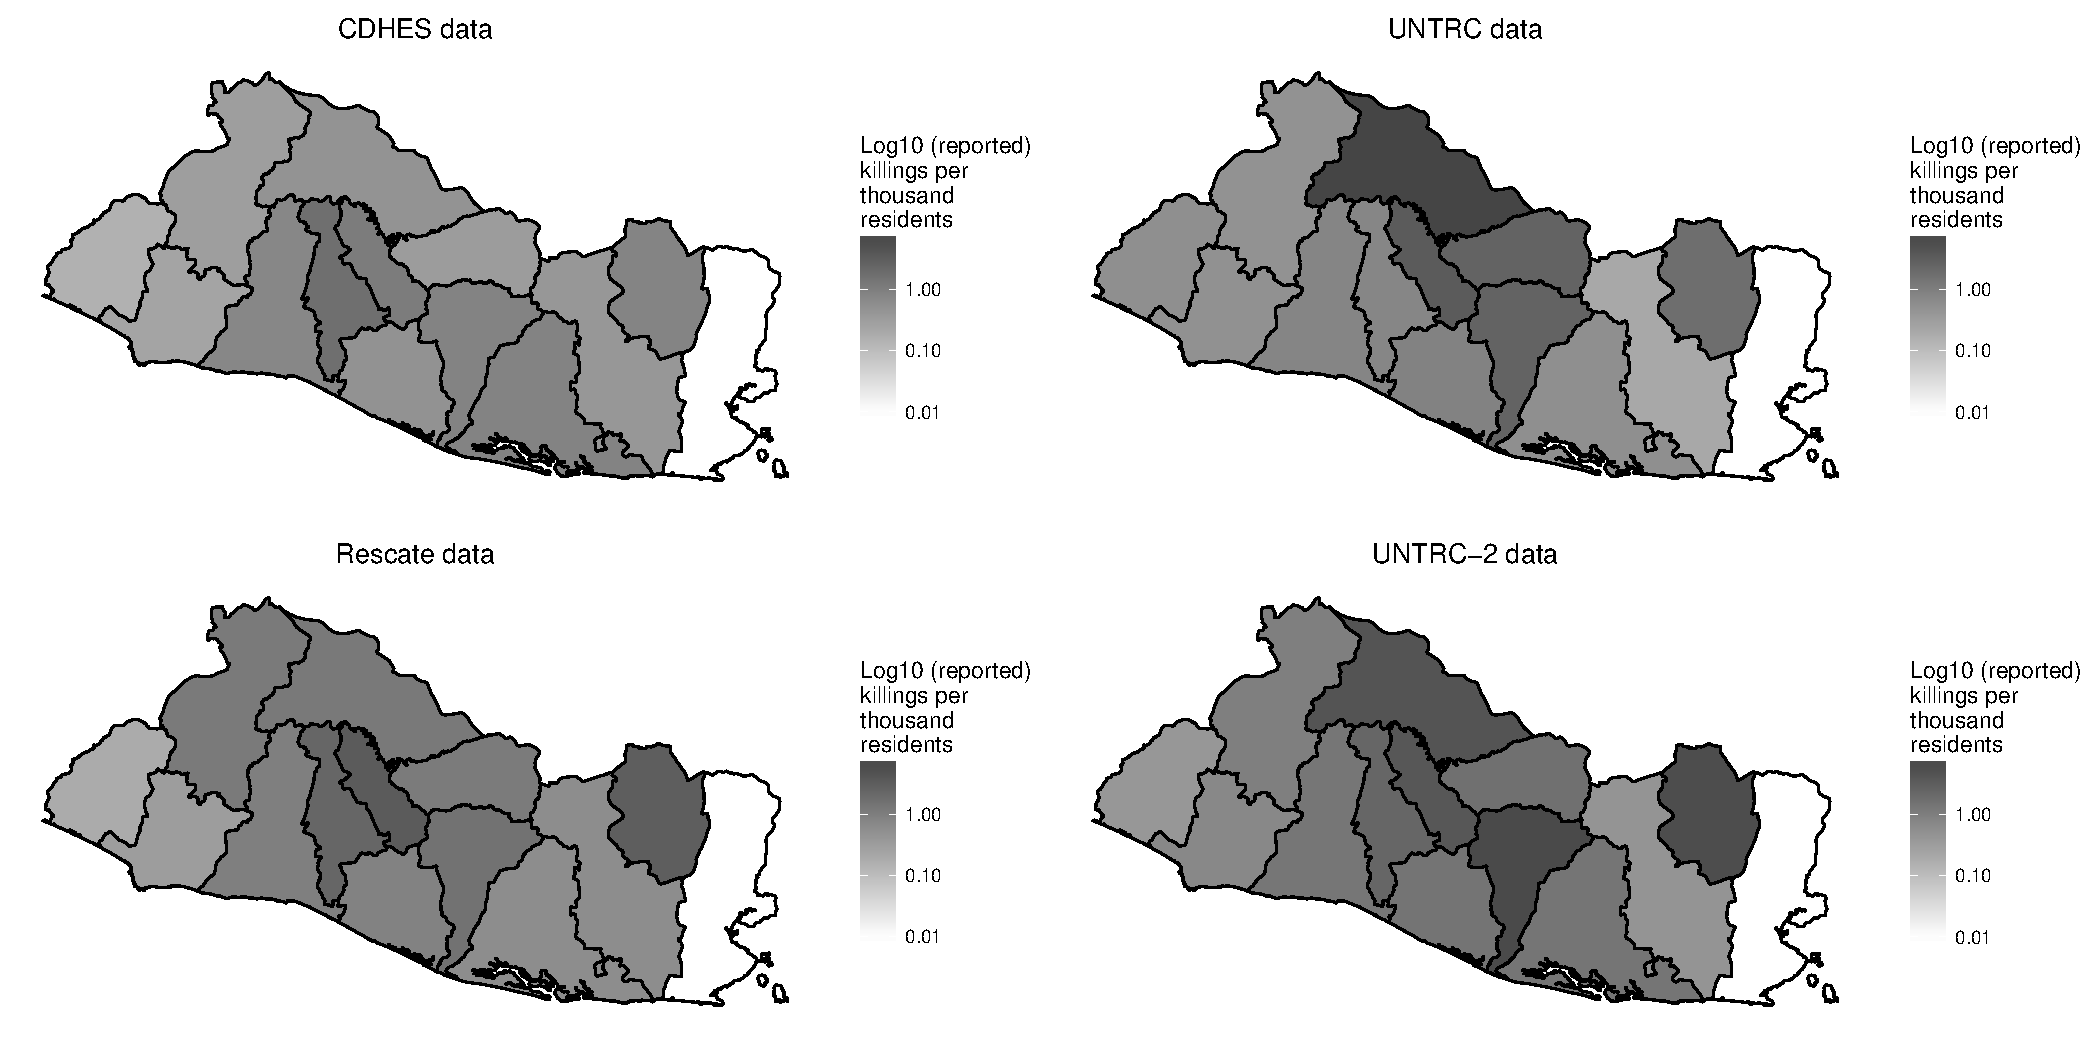
\includegraphics{../input/lethals-by-dept-raw-fig.pdf}
\caption{Log per-capita lethal violence, four datasets.}
\end{figure}

\begin{figure}
\centering
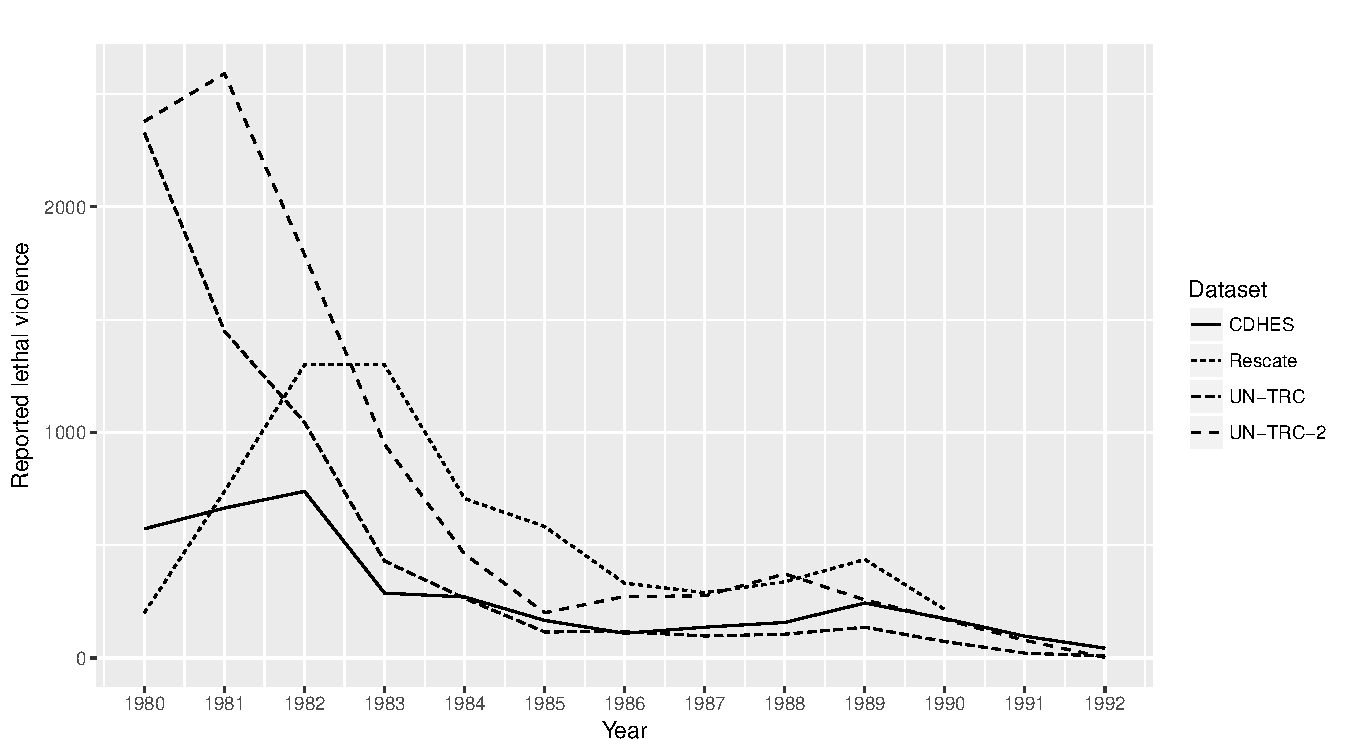
\includegraphics{../input/lethals-by-yr-raw-fig.pdf}
\caption{Lethal violence by year, four datasets.}
\end{figure}

\begin{figure}
\centering
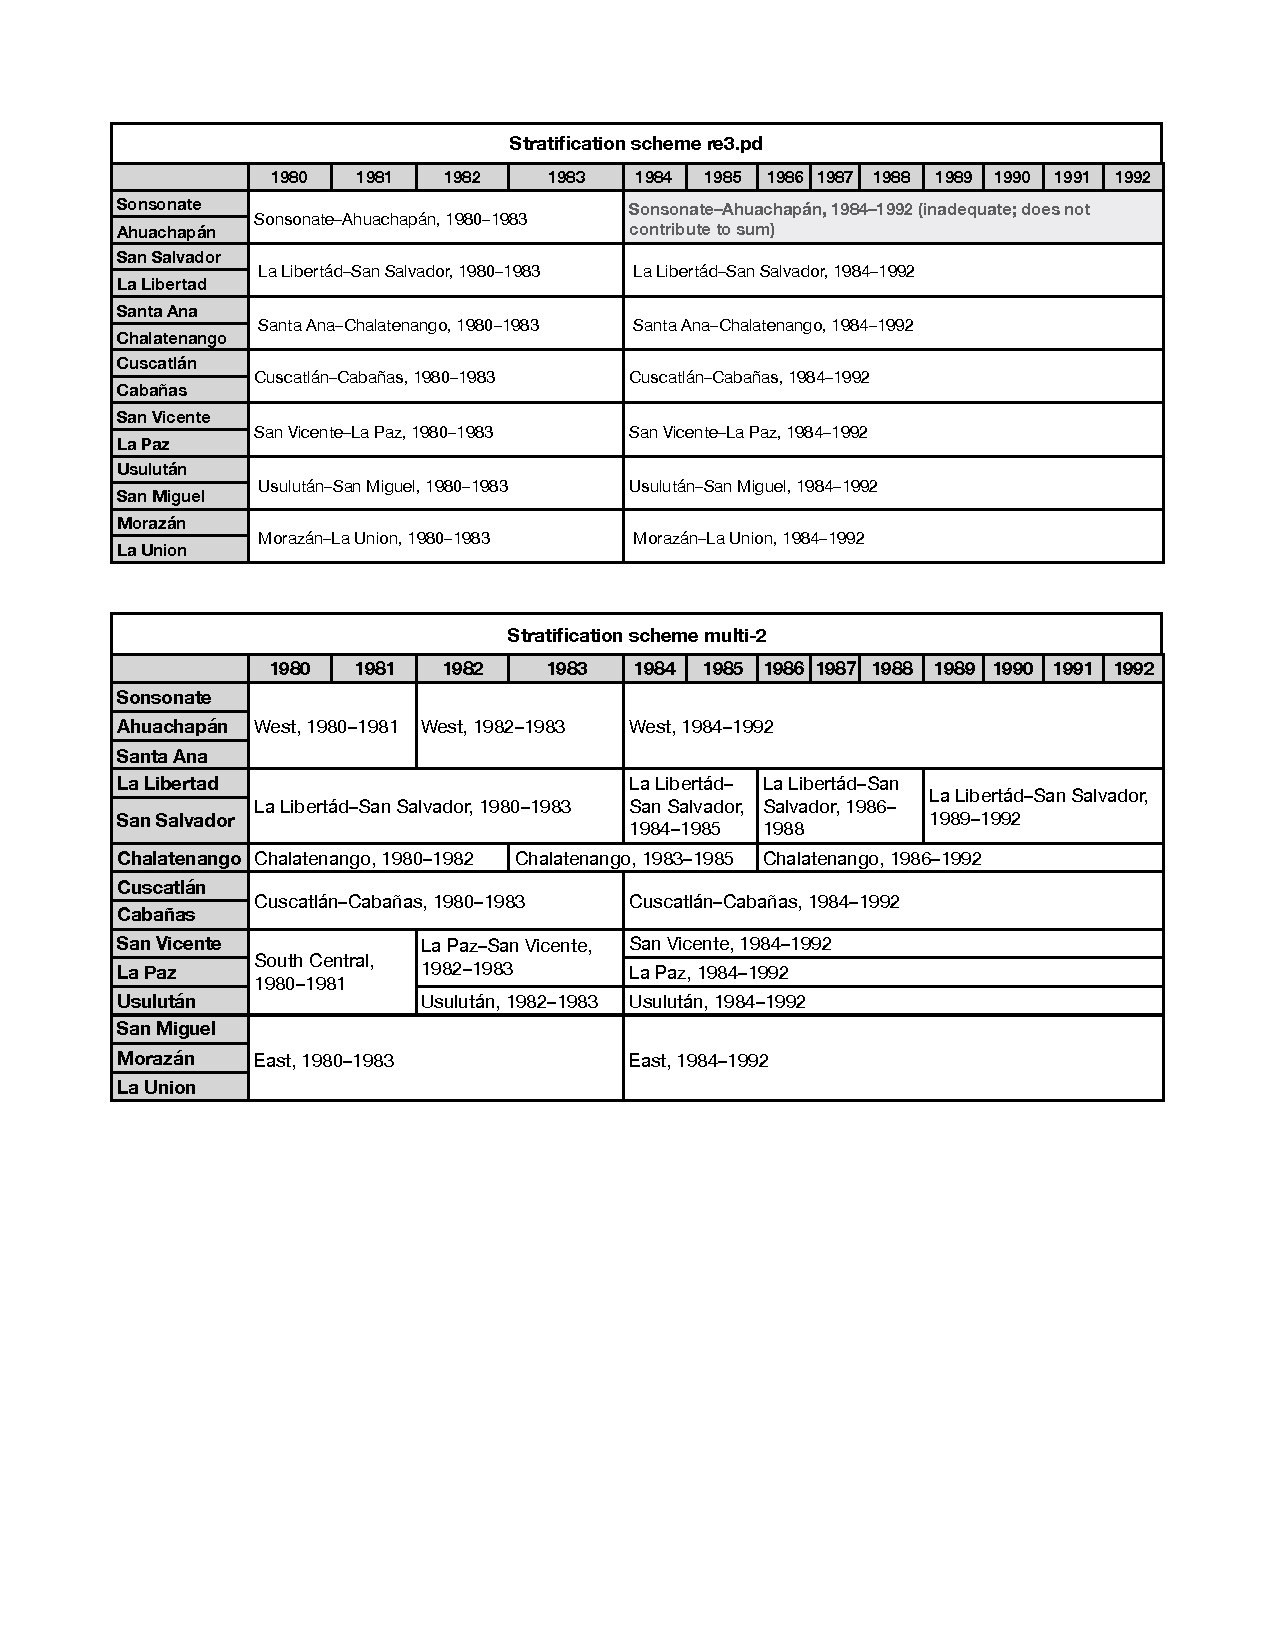
\includegraphics{../input/strata.pdf}
\caption{Stratifications underlying two global sums}
\end{figure}

\begin{figure}
\centering
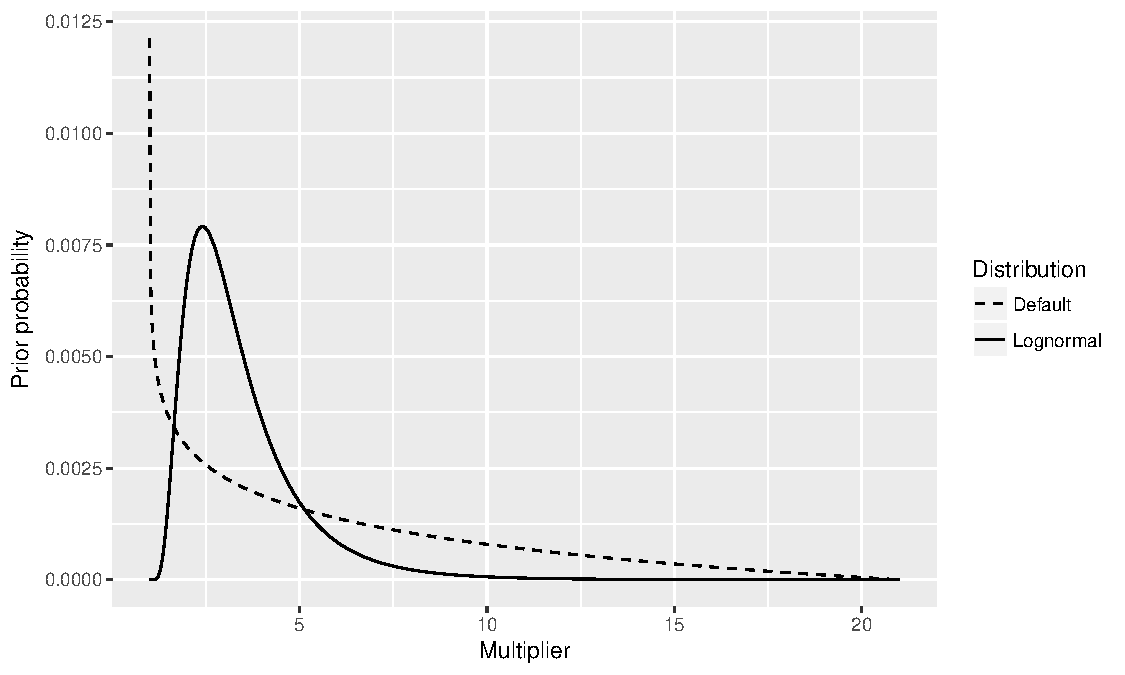
\includegraphics{../input/prior-comparison-fig.pdf}
\caption{Prior probabilities using default and Lognormal (0.7,0.6)
distributions}
\end{figure}

\begin{figure}
\centering
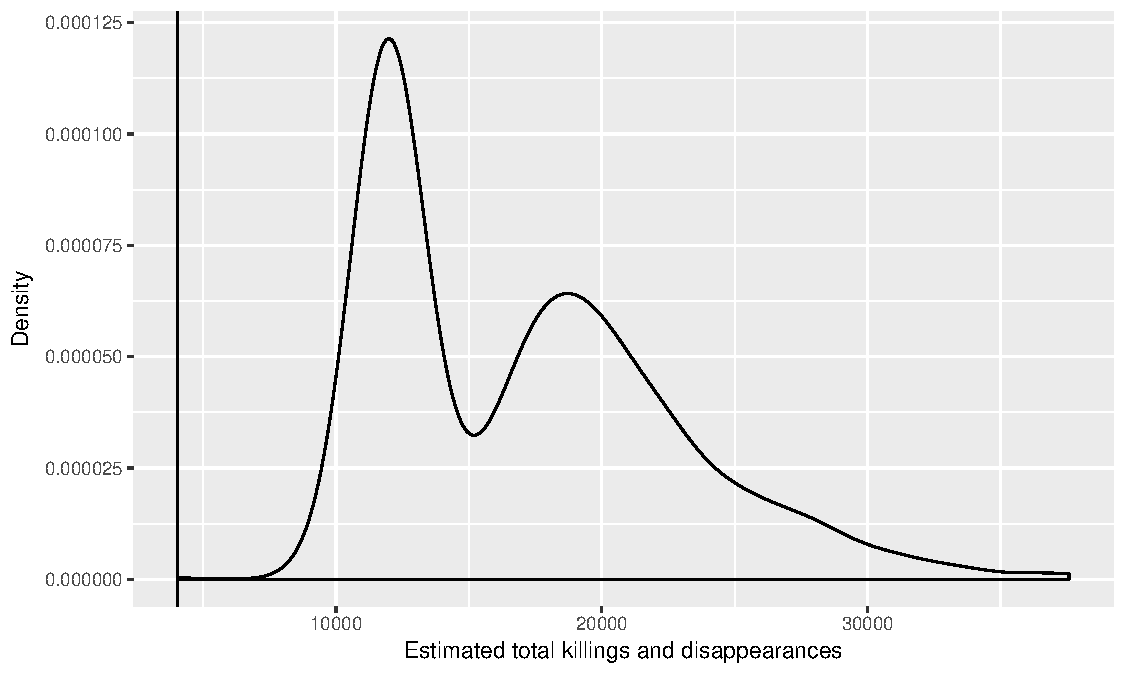
\includegraphics{../input/post-prob-1981-fig.pdf}
\caption{Posterior probability of estimated total killings for 1981}
\end{figure}

\begin{figure}
\centering
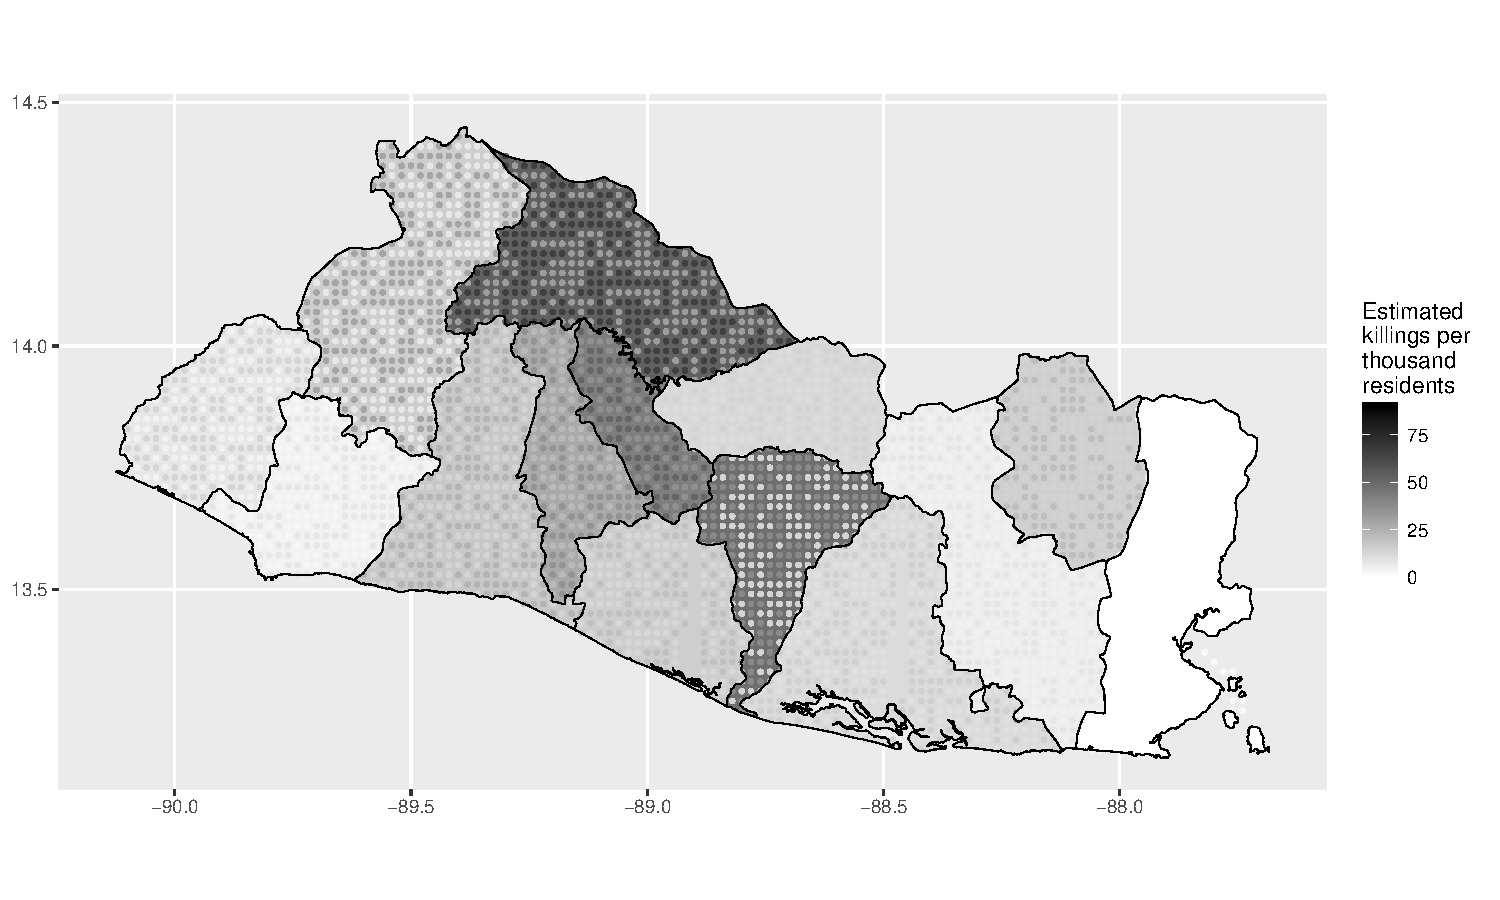
\includegraphics{../input/lethals-by-dept-est-fig.pdf}
\caption{Killings and disappearances by department, MSE estimates.}
\end{figure}

\begin{figure}
\centering
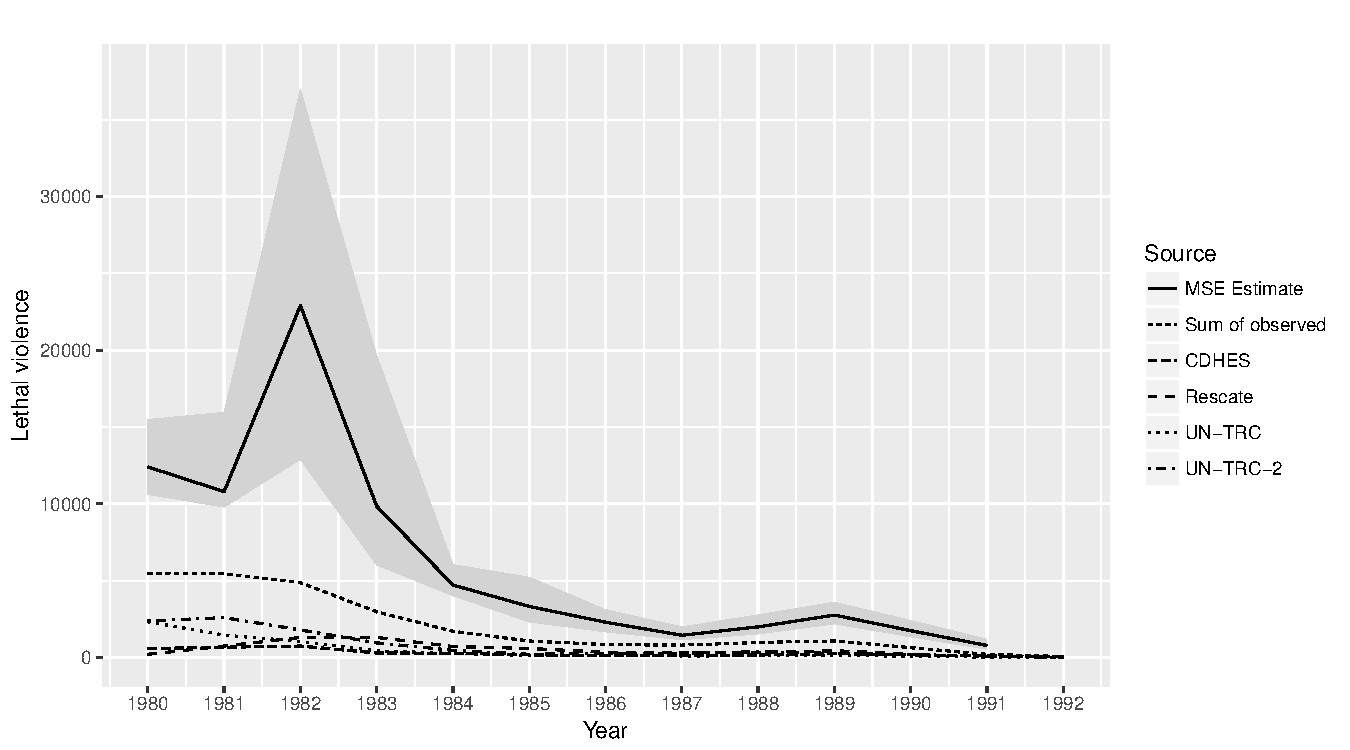
\includegraphics{../input/lethals-by-yr-est-fig.pdf}
\caption{Lethal violence by year, raw data and MSE estimates.}
\end{figure}

\begin{figure}
\centering
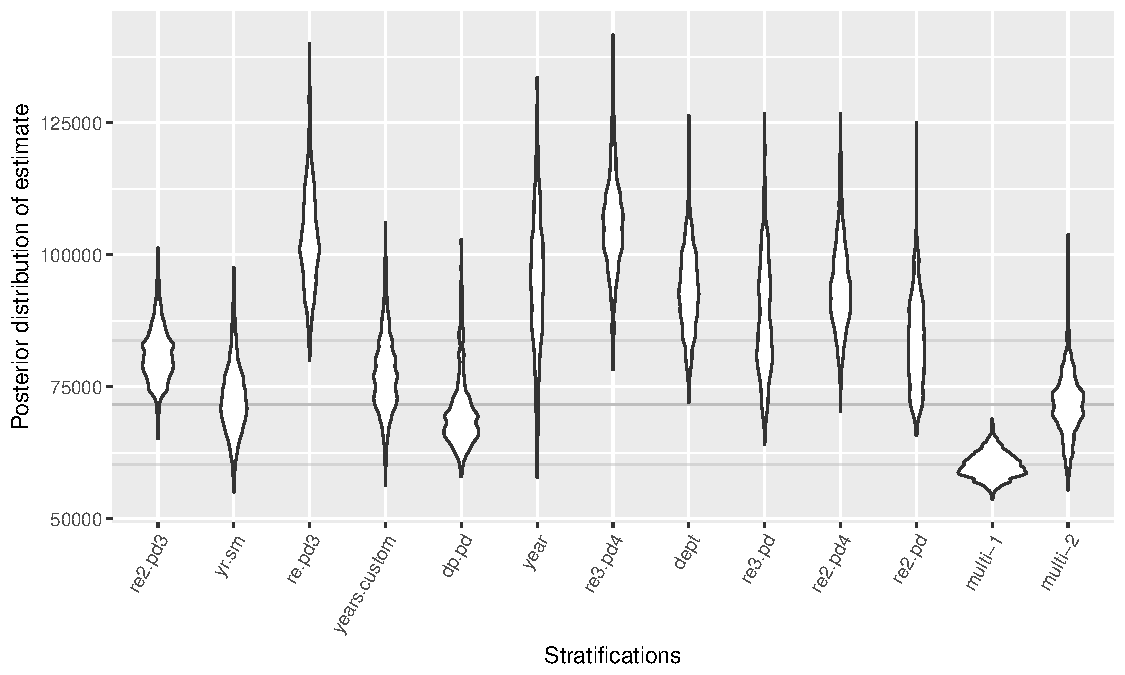
\includegraphics{../input/post-prob-violins-fig.pdf}
\caption{Posterior probabilities for sums across multiple
stratifications}
\end{figure}

\begin{figure}
\centering
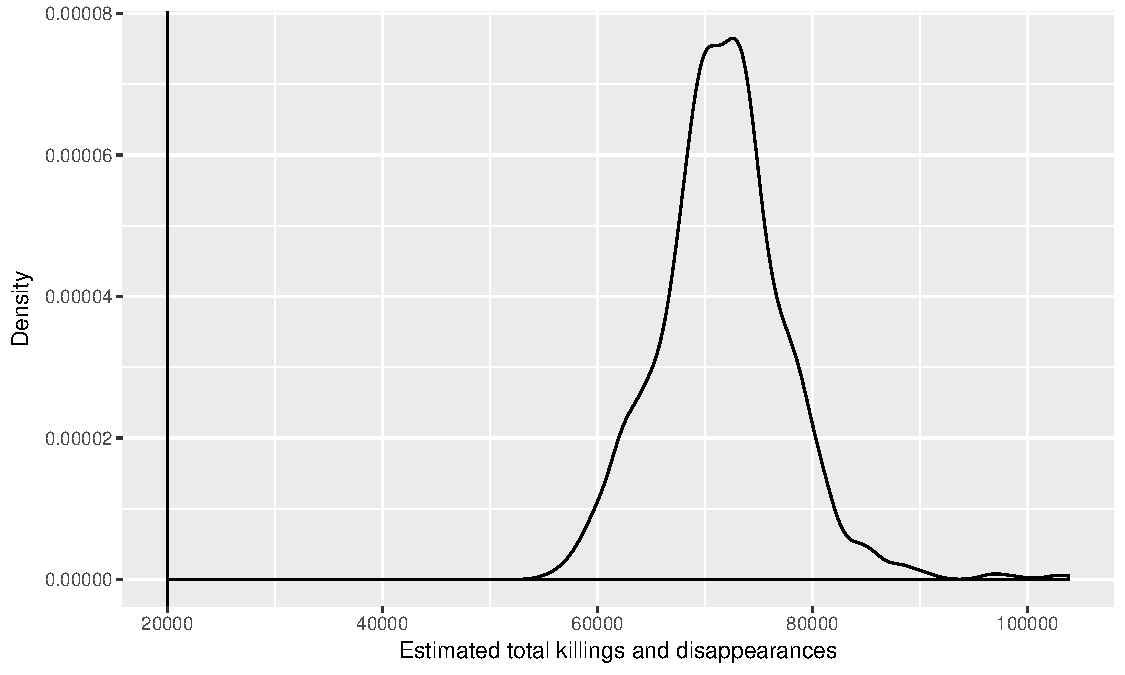
\includegraphics{../input/post-prob-multi2-fig.pdf}
\caption{Posterior probability of estimated killings in El Salvador,
1980-1991, for stratification ``multi-2''}
\end{figure}


\end{document}
